% !Mode:: "TeX:UTF-8:Hard"
\ifx \allfiles \undefined
\documentclass[a4paper,12pt,twoside]{book}
%\usepackage{CJKutf8}
\usepackage[T1]{fontenc}
\usepackage{pifont}
\usepackage{graphicx}
\usepackage{multirow} 
\usepackage{longtable}
\usepackage{capt-of}
\usepackage{color}
\usepackage{amsmath}

\newcommand{\linuxcommand}[1]{\texttt{\textcolor{blue}{\$ #1 \Pisymbol{psy}{191}}}}
\newcommand{\op}[1]{\textcolor{blue}{-#1}}
\newcommand{\hotkey}[1]{\framebox{#1}}
\newenvironment{screen}{\sffamily}{\rmfamily}

% for C/C++ frame box
\usepackage{listings}
\definecolor{mygray}{rgb}{0.9,0.9,0.9}
\lstset{ %
  backgroundcolor=\color{mygray}, basicstyle=\small
}
\lstset{morecomment=[s][\color{red}]{/*-}{*/}}
\newcommand{\Hilight}[1]{\makebox[0pt][l]{\color{yellow}\rule[-3pt]{#1em}{11pt}}}
\newcommand{\HilightLine}[2][yellow]{\makebox[0pt][l]{\color{#1}\rule[-4pt]{#2em}{13.9pt}}}

\newenvironment{answer}{\ttfamily}{\par}

\newcommand{\specialcell}[2][c]{%
  \begin{tabular}[#1]{@{}c@{}}#2\end{tabular}}

\begin{document}
%\begin{CJK*}{UTF8}{song}
\title{Data Structure, algorithm}
\author{yan zhao}
\date{}\maketitle

\else
\chapter{Data Structure, algorithm} 
\fi

\chapter{Data Structure}



\section{Basic Knowledge}
\begin{itemize}
\item Data structure is known as ADT,  which is independent of implementation. For example, stack can be implemented by array or linked list. Such as stack in STL library, It's implemented by deque default.   

\item \textbf{Linear and hierarchical structures}. Array, linked lists, stacks and queue are linear structures. And tree, graph, heaps are hierarchical.

\item STL is a good reference when you learn data structure, especially interface of STL container. such as \texttt{push}, \texttt{pop}  and \texttt{top} for stack and \texttt{priority\_queue}. For queue, besides push() pop(),  there are also front() and back(). Just remember four words: \textbf{push pop front back}

\item All the normal container(not including adapter container, stack, queue, priority\_queue) includes four basic operations: begin(), end(), insert() and erase(). 

\item Big O notation. Remember below English words: constant, logarithmic (log n), linear (n)  linearithmic (n*log(n)) , quadratic $2^{n}$, polynomial(quadratic cubic),  exponential $c^{n}$.  factorial $n!$.  O($10^{N}$): trying to break a password by testing every possible combination (assuming numerical password of length N).  traveling saleman problem(TSP)is factorial $n!$. 
\end{itemize}


\section{Array}
\subsubsection{basic}
\begin{itemize}
\item All language support array and think it as build-in data type.  
\begin{lstlisting}[frame=single, language=c++]
//C/C++ language
int a[3]; or int a[4][5].  
STL vector<int> (4,0);
  
//C# language 
object[] a1 = {"string", 123, true};
\end{lstlisting}

\item Array support three basic operations: Index, insert, delete(erase in STL).  

\item Dynamic two dimension array can be implemented below:  char ** p; should be used as ragged array. Pay attention to p[1][2] and pa[1][2]. They are all correct forms.

\item All ragged array should include terminate flag, so you can know the length of each row.  For C-style string ragged array, the 'NULL' in the end of string can be used as terminate flag directly, so ragged array is idea container for C-style string array. 

\begin{lstlisting}[frame=single, language=c++]
char **p;
char* a[]={"zhao","yan","hello"};
p = a;
printf("%c\n",*(*(p+1)+2)); //p[1][2]

int (*pa)[3];
int aa[2][3] = {{1,2,3},{4,5,6}};
pa = aa;
printf("%d\n",pa[1][2]);//*(*(pa+1)+2);
\end{lstlisting} 

\item If you want to insert an element into an array, you  \textbf{need to copy backward from end. }
if erase an element from an array, \textbf{copy forward from erasing point.}

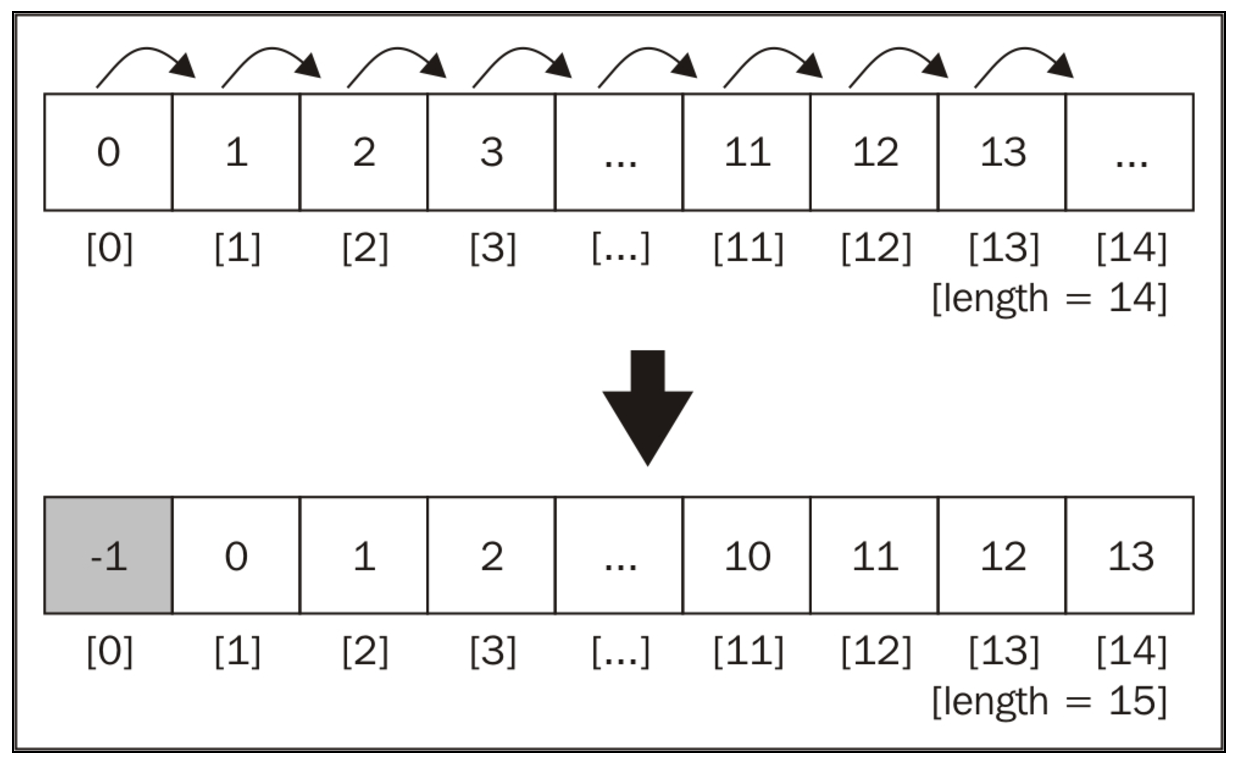
\includegraphics[scale=0.35]{pics/array_insert.png} \newline

\item If you have an array of big object, and you need to sort it. You can build a array of pointer to point to each object in the array. When you sort the an array of big object,  you just move pointer instead, It is called "indirect addressing", It can help you to avoid moving big chunk of data.  If you want to put them into STL container, you can use smart pointer, such as unique\_ptr. Don't use auto\_ptr. 

\item reverse array can be implemented by swap, But reverse list need different algorithm, so in STL , list<> has its own reverse member function. 
\begin{lstlisting}[breaklines]
1) Initialize start and end indexes. 
	start = 0, end = n-1
2) In a loop, swap arr[start] with arr[end] and change start and end as follows.
	start = start + 1;  end = end - 1
\end{lstlisting}

\item Write a function rotate(ar[], d, n) that rotates arr[] of size n by d elements.
\begin{enumerate}
\item single rotate method
\begin{lstlisting}[breaklines]
leftRotate(arr[], d, n)
start
  For i = 0 to i < d
    Left rotate all elements of arr[] by one
end
//***********************//
To rotate by one, store arr[0] in a temporary variable temp, move arr[1] to arr[0], arr[2] to arr[1] ... and finally temp to arr[n-1]
\end{lstlisting}
\item reverse method
\begin{lstlisting}[breaklines]
rotate(arr[], d, n)
  reverse(arr[], 1, d) ;
  reverse(arr[], d + 1, n);
  reverse(arr[], l, n);
\end{lstlisting}
\textbf{Idea: middle part reverse twice, so keep origin value}


\item you can use rotate in insert sort method. also use in slide. Detail can be found in "Top 5 Beautiful C++ std Algorithms Examples"
\begin{lstlisting}[breaklines]
for (auto i = start; i != end; ++i)
std::rotate(std::upper_bound(start, i, *i), i, std::next(i));


template <typename It> 
auto slide(It f, It l, randIter p) -> std::pair<It, It>{
	if (p < f) return { p, std::rotate(p, f, l) };
	if (l < p) return { std::rotate(f, l, p), p };
	return { f, l };
}
\end{lstlisting}



\end{enumerate}

\end{itemize}

\subsection{Application}
\begin{itemize}

\item Given an array A[] and a number x, check for pair in A[] with sum as x. 
\begin{enumerate}
\item Answer 1: Sort O(n*log(n))
\begin{lstlisting}[breaklines]
hasArrayTwoCandidates (A[], ar_size, sum)
1) Sort the array in non-decreasing order.
2) Initialize two index variables to find the candidate 
   elements in the sorted array.
       (a) Initialize first to the leftmost index: l = 0
       (b) Initialize second  the rightmost index:  r = ar_size-1
3) Loop while l < r.
       (a) If (A[l] + A[r] == sum)  then return 1
       (b) Else if( A[l] + A[r] <  sum )  then l++
       (c) Else r--    
4) No candidates in whole array - return 0
\end{lstlisting}
\textbf{Idea: Don't need keep index information, so you can sort it. }
\item Answer 2: Hash O(n)
\end{enumerate}

\item Count triplets with sum smaller than a given value. 
\begin{lstlisting}[breaklines]
1) Sort the input array in increasing order. 
2) Initialize result as 0.
3) Run a loop from i = 0 to n-2.  An iteration of this loop finds all
   triplets with arr[i] as first element.
     a) Initialize other two elements as corner elements of subarray \newline
        arr[i+1..n-1], i.e., j = i+1 and k = n-1
     b) Move j and k toward each other until they meet, i.e., while (j < k)\newline
            (i) if (arr[i] + arr[j] + arr[k] >= sum), then do k-- 

            // Else for current i and j, there can (k-j) possible third elements 
            // that satisfy the constraint.\newline
            (ii) Else Do ans += (k - j) followed by j++ 
\end{lstlisting}
\textbf{Idea: Same Idea as previous question, Don't need keep index information, so you can sort it. }


\item Given an array of positive integers. All numbers occur even number of times except one number which occurs odd number of times. Find the number in O(n) time and constant space.
Example: I/P = [1, 2, 3, 2, 3, 1, 3] and O/P = 3. 
\begin{lstlisting}[breaklines]
The Best Solution is to do bitwise XOR of all the elements. XOR of all elements gives us odd occurring element. Please note that XOR of two elements is 0 if both elements are same and XOR of a number x with 0 is x.
\end{lstlisting}
\textbf{Idea: Perform some calculation on all elements. }


\item You are given a list of n-1 integers and these integers are in the range of 1 to n. There are no duplicates in list. One of the integers is missing in the list. Write an efficient code to find the missing integer.
\begin{lstlisting}[breaklines]
1) Get the sum of numbers 
       total = n*(n+1)/2
2  Subtract all the numbers from total and you will get the missing number.
\end{lstlisting}
\textbf{Idea: Perform some calculation on all elements. }

\item Max product of the three numbers for a given array of size N. 
\begin{lstlisting}[breaklines]
Find the three largest numbers in the array (n1, n2, n3) and the two smallest numbers (m1, m2). The answer is either n1 x n2 x n3 or n1 x m1 x m2
\end{lstlisting}
\textbf{Idea: Not sort, but nth max element based on heap}

\item Given an unsorted array of non-negative integers, find a \textbf{continuous} subarray which adds to a given number.  Examples: Input: arr[] = {1, 4, 20, 3, 10, 5}, sum = 33; Ouptut: Sum found between indexes 2 and 4
\begin{lstlisting}[breaklines]
Initialize a variable curr\_sum as first element. curr\_sum indicates the sum of current subarray. Start from the second element and add all elements one by one to the curr\_sum. If curr\_sum becomes equal to sum, then print the solution. If curr\_sum exceeds the sum, then remove trailing elemnents while curr\_sum is greater than sum.
\end{lstlisting}
\textbf{Idea: 1) You must keep index information, so you can't sort.  keep head and trail two index}

\item An element in a sorted array can be found in O(log n) time via binary search. But suppose we rotate an ascending order sorted array at some pivot unknown to you beforehand. So for instance, 1 2 3 4 5 might become 3 4 5 1 2. Devise a way to find an element in the rotated array in O(log n) time.

The basic idea is DC(divided conquer.) 
\begin{enumerate}
	\item Use DC, The first part is end condition. For this question, the end atomic condition is e-b ==1(only two elements in it)
	\item If use array, better use index directly.
	\item When you have last atomic condition, you need to decide boundary  b, (e-b)/2, e. \textbf{When you decide boundary boundary, you have to make half part of contents still includes answer. That is very useful hint for you to decide boundary value}
\end{enumerate}

\begin{lstlisting}[breaklines]
size_t find_rot(const vector<int> &vi, int b, int e){
	if (e-b ==1){
		return b;
		
	}
	int pivot = b + (e-b)/2;
	cout<<"pivot"<<pivot<<endl;
	if (vi[b]<vi[pivot]){
		return find_rot(vi, pivot, e);
	}
	else{
		return find_rot(vi, b, pivot);
	}
}
\end{lstlisting}

\item Binary search. The basic idea is DC(divided conquer.) 
\begin{enumerate}
	\item Use DC, The first part is end condition. For this question, the end atomic condition is e==b. if search may return -1(not found), then (e-b)/2 should also be included in the recursive call
	\item If use array, better use index directly.
	\item \textbf{if you use index, you need change pivot into index: pivot = b+(e-b)/2;}
	\item When you have last atomic condition, you need to decide boundary  b, (e-b)/2, e. \textbf{When you decide boundary, you have to make half part of contents still includes answer. That is very useful hint for you to decide boundary value}
	\item because -1 is valid answer, so you should call 
	b\_f(vi, b, pivot, value), not b\_f(vi, b, pivot-1, value), please pay attention here. 
	

\end{enumerate}

\begin{lstlisting}[breaklines]
int b_f(const vector<int> &vi, int b, int e, int value){
	if(b == e){
		return vi[b]!=value ? -1 : b;
	}
	int pivot = b+(e-b)/2; //(b+e)/2 
						   //b/2+e/2 + a&b&1
	cout<<"pivot"<<pivot<<endl;
	if(vi[pivot] == value){
		return pivot;
	}
	else if (vi[pivot]>value){
		return b_f(vi, b, pivot, value);
	}
	else{
		return b_f(vi, pivot, e, value);
	}
}
\end{lstlisting}



\item Given an array arr[] of integers, find out the difference between any two elements such that larger element appears after the smaller number in arr[]. Examples: If array is [2, 3, 10, 6, 4, 8, 1] then returned value should be 8 (Diff between 10 and 2). If array is [ 7, 9, 5, 6, 3, 2 ] then returned value should be 2 (Diff between 7 and 9)
\begin{lstlisting}[breaklines]
In this method, instead of taking difference of the picked element with every other element, we take the difference with the minimum element found so far. So we need to keep track of 2 things:
1) Maximum difference found so far (max\_diff).
2) Minimum number visited so far (min\_element).
\end{lstlisting}
\textbf{Keep position, but this problem can be divided by sub-problem. Such as, [ 7, 9, 5, 6, 3, 2 ] can be seen as [7,9] [5, 6] [3] [2]  Once current element is less than min\_element, begin a new sub-problem.}

\item Write a program to print all the LEADERS in the array. An element is leader if it is greater than all the elements to its right side. And the rightmost element is always a leader. For example int the array {16, 17, 4, 3, 5, 2}, leaders are 17, 5 and 2. 
\begin{lstlisting}[breaklines]
Scan all the elements from right to left in array and keep track of maximum till now. When maximum changes it's value, print it.
\end{lstlisting}
\textbf{Same idea just like previous}

\item Inversion Count for an array indicates -- how far (or close) the array is from being sorted. If array is already sorted then inversion count is 0. If array is sorted in reverse order that inversion count is the maximum. Formally speaking, two elements a[i] and a[j] form an inversion if a[i] > a[j] and i < j. Example:
The sequence 2, 4, 1, 3, 5 has three inversions (2, 1), (4, 1), (4, 3).

\begin{lstlisting}[breaklines]
1) Create an empty Set in C++ STL (Note that a Set in C++ STL is 
   implemented using Self-Balancing Binary Search Tree). And insert
   first element of array into the set.

2) Initialize inversion count as 0.

3) Iterate from 1 to n-1 and do following for every element in arr[i]
     a) Insert arr[i] into the set.
     b) Find the first element greater than arr[i] in set
        using upper_bound() defined Set STL.
     c) Find distance of above found element from last element in set
        and add this distance to inversion count.

4) Return inversion count.
\end{lstlisting}

\begin{lstlisting}[breaklines]
int main()
{
	vector<int> vi = {2, 4, 1, 3, 5};
	set<int> si;
	int sum = 0;
	for(auto i :vi){
		si.insert(i);
		cout<<i<<endl;
		auto it1 = si.upper_bound(i);
		if (it1 != si.end())
		cout<<"***"<<*it1<<endl;
		sum += distance(it1, si.end());
	}
	
	cout<<sum<<endl;
	cout<<"Hello World";
	
	return 0;
}
\end{lstlisting}
\begin{description}
	\item[line ] \textbf{set also support iterator, it will output sorted element from begining to end }
	\item[line ] \textbf{distance function, you have to input smaller iterator first. for set, if you input end, it will fall into dead loop}
	
\end{description}

\textbf{1) You need keep index(position) information. (No sort, no calculation).  2) you can't divid it to subj-problem. 3) You have to use auxiliary DS outside. such as set. which store how many element is greeter than current element.  }


\item Convert array into Zig-Zag fashion ? The converted array should be in form a < b > c < d > e < f. 
\begin{lstlisting}[breaklines]
We can convert in O(n) time using an Efficient Approach. The idea is to use modified one pass of bubble sort. Maintain a flag for representing which order(i.e. < or >) currently we need. If the current two elements are not in that order then swap those elements otherwise not.
Let us see the main logic using three consecutive elements A, B, C. Suppose we are processing B and C currently and the current relation is '<'. But we have B > C. Since current relation is '<' previous relation must be '>' i.e., A must be greater than B. So, the relation is A > B and B > C. We can deduce A > C. So if we swap B and C then the relation is A > C and C < B. Finally we get the desired order A C B
\end{lstlisting}


\item Conclusion: Main methods for array questions. 
\begin{enumerate}
\item Clue1: Get max and min value, based on heap, init a heap need O(n), when you get the second largest or third largest one, you only need O(log(n)). It's better than sort O(n*log(n) ). 



\item Clue2: Sort
\item Clue3: For continuous subarray, keep head and trail two index.
\item Clue4: Calculate, such as sum and bit operator XOR. 
\item Clue5: Use other auxiliary DS, such as, map, set or hash\_map.  They can be used as count and sort. 
\end{enumerate}

\end{itemize}

\section{Linked list}
\subsection{Basic}
\begin{itemize}
\item list in STL is bidirectional list(double-linked), in C++11, you can use forward\_list as single-linked list. 

\item CreateList, DeleteList, Length, InsertItem, DeleteItem, 
\item  Declaration of Linked list. 
\begin{lstlisting}[frame=single, language=c++]
//C 
struct node{ 
int a; 
 struct node* link
} ;

//C++
Template <class T>
Class ChainNode{
   friend Chain<T>;
   T data
  ChainNode<T> *link;
}

template<class T>
class Chain{
......
ChainNode<T> *head;
}
\end{lstlisting}
\end{itemize}

\subsection{Operations}
\begin{itemize}
\item insert, \textbf{get an index to previous pointer}
\begin{lstlisting}[frame=single, language=c++, mathescape=true]
//Consider if it's the first element. 
Insert(int k, const T &x)
chainNode<T> *i = new chainNode<T> (x);

$\Hilight{15}$ //leftside is pointer pointed direction
$\Hilight{15}$ //rightside is node, but in list, all nodes only 
$\Hilight{15}$ //can be accessed by a pointer.
$\Hilight{15}$ //insert after p node (with new drawing pad, draw picture here.)
i->link = p->link;
p->link = i;
// i is inserted element, p is position.  
//You can remember i=p p=i  and fore three links.
\end{lstlisting}

\item insert, before p node, what should I do?  \textbf{Just swap two node, then deal with next node. Don't touch next node in one atomic action. That is rule. }
\begin{lstlisting}[frame=single, language=c++, mathescape=true]
1)create temp auto node, new a i node.
 
while(p->link) 
2) copy value from p to temp node
3) copy value i to p.
4) copy temp value to i value
p = p->link.  
\end{lstlisting}

\item delete \textbf{get an index to previous pointer}
\begin{lstlisting}[frame=single, language=c++]
Delete(int k, const T&x)
d = p->link;
p->link = d->link ;
delete d;
//d=p p=d and last three links
\end{lstlisting}

\item Indirect addressing combines array and list. You should store pointer in array, and each pointer refer to random storage object. A typical usage is char* [] each item in array is char*(string), when you sort the strings, you just move pointers. It will save a lot of move time.  
\item In C\#, it really support Generic List List<T> and nongeneric ArrayList. 
\begin{lstlisting}[frame=single, language=c++]
List<string> words = new List<string>();
words.Add("avocado");
\end{lstlisting}

\end{itemize} 

\subsection{Application}
\subsubsection{Bucket sort}

\begin{itemize}
\item For each item, the value range is limited, and is integer. For example, sort all students score. (0<=score<=100). 
\item Basic step:  Here, Link list is best option to implement a bucket. Because Nobody will now how many elements will be put into the each bucket. 
\begin{enumerate}
\item Set up an array of initially empty "buckets".
\item Scatter: Go over the original array, putting each object in its bucket. 
\item Sort each non-empty bucket.(Optional )
\item Gather: Visit the buckets in order and put all elements back into the original array.
\end{enumerate}

\end{itemize}

\subsubsection{Radix sort}

\begin{itemize}
\item r is radix, $x\%r, (x\%r^{2})/r, (x\%r^{3})/r^{2}$  get each digit from least significant digit (LSD) radix sorts to most significant digit. 

\begin{lstlisting}[frame=single, language=c++]
int i ;
int k;
while(i%10){
k = i%10;
i = i/10;
}
\end{lstlisting}


\begin{enumerate}
\item according to r, prepare two arrays buckets A, B. 
\item Sort according to one position and put them into A array buckets. 
\item loop through A array buckets, and get next position digit. and then according to its value put into B array buckets.
\item swap A,B two array, then goto step 2.
\end{enumerate}

\end{itemize}

\subsubsection{Online Equivalence class}
\begin{itemize}
\item definition of Equivalence relationship
\begin{enumerate}
\item a ~ a. (Reflexivity)
\item a ~ b if and only if b ~ a. (Symmetry)
\item if a ~ b and b ~ c then a ~ c. (Transitivity)
\end{enumerate}

\item online equivalence class, also known union-find question.  
\begin{enumerate}
\item method 1: use array  \newline 
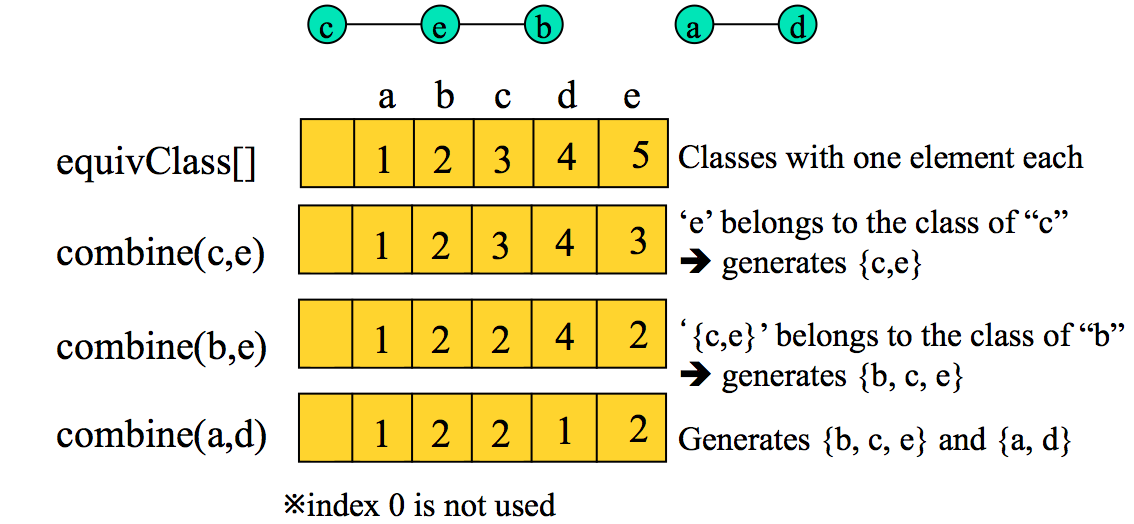
\includegraphics[scale=0.55]{pics/online_1.png} 

\item method 2: stimulate pointer \newline 
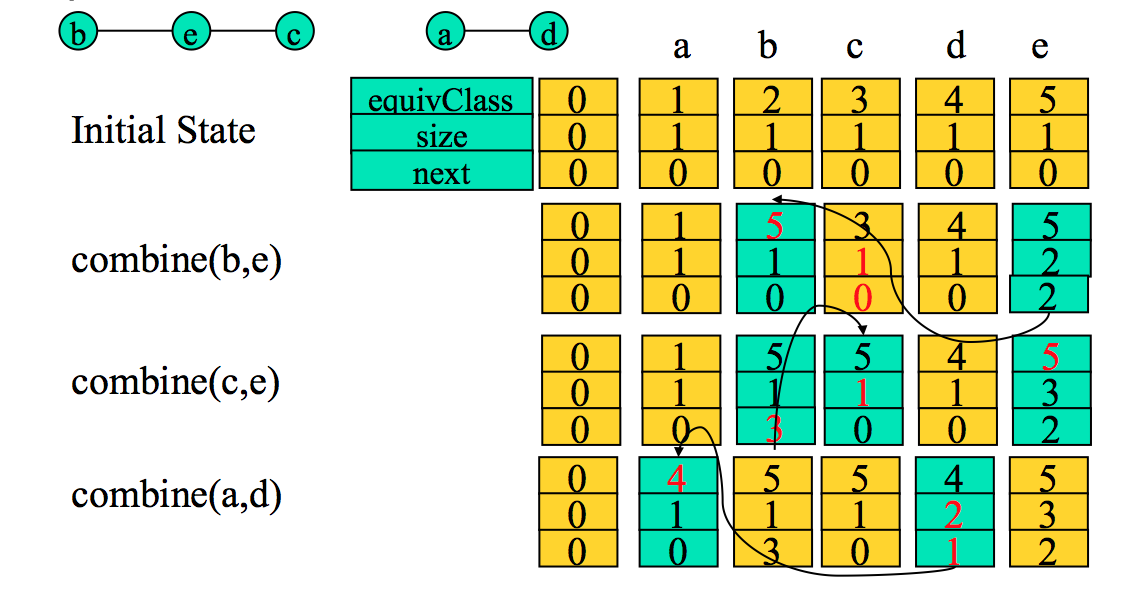
\includegraphics[scale=0.55]{pics/online_2.png}  
\end{enumerate}

\end{itemize}

\subsubsection{Offline Equivalence class}
\begin{itemize}
\item offline equivalence class, known n and R, get all Equivalence class.  
\item Two phases to determine equivalence class
Phase 1: Equivalence pairs (i, j) are read in and adjacency (linked) list of each object is built.
Phase 2: Trace (output) the equivalence class containing object i with stack (depth-first search). Next find another object not yet output, and repeat.

\begin{lstlisting}[frame=single, language=c++]
for (int i = 1; i <= n; i++)  // output equivalence classes
   if  (!out[i]) { // start of a new class
             out[i] = true;
             unprocessedList.push(new Integer(i)) ;
    while (!unprocessedList.empty()) { // get rest of class from unprocessedList
          int j = ((Integer) unprocessedList.pop()).intValue();
           while  (!list[j].empty()) { // elements on list[j] are in the same class
                  int q = ((Integer) list[j].pop()).intValue();
                  if (!out[q]) { // q not yet output
                      System.out.print(q + " ");
                      out[q] = true;
                      unprocessedList.push(new Integer(q));  } //end of if
               } //end of while
            }  //end of while 
        } //end of if

\end{lstlisting}

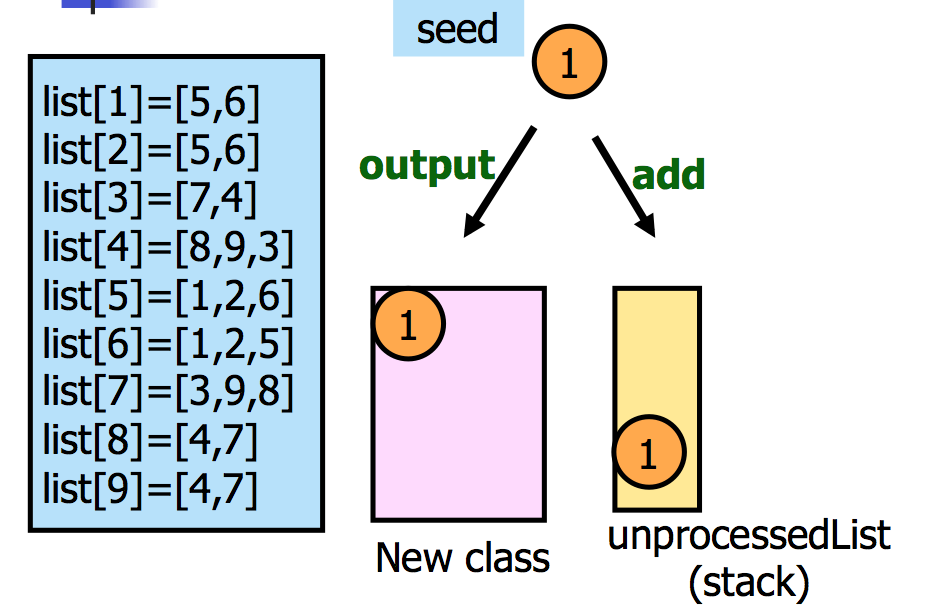
\includegraphics[scale=0.35]{pics/offline_1.png} \newline
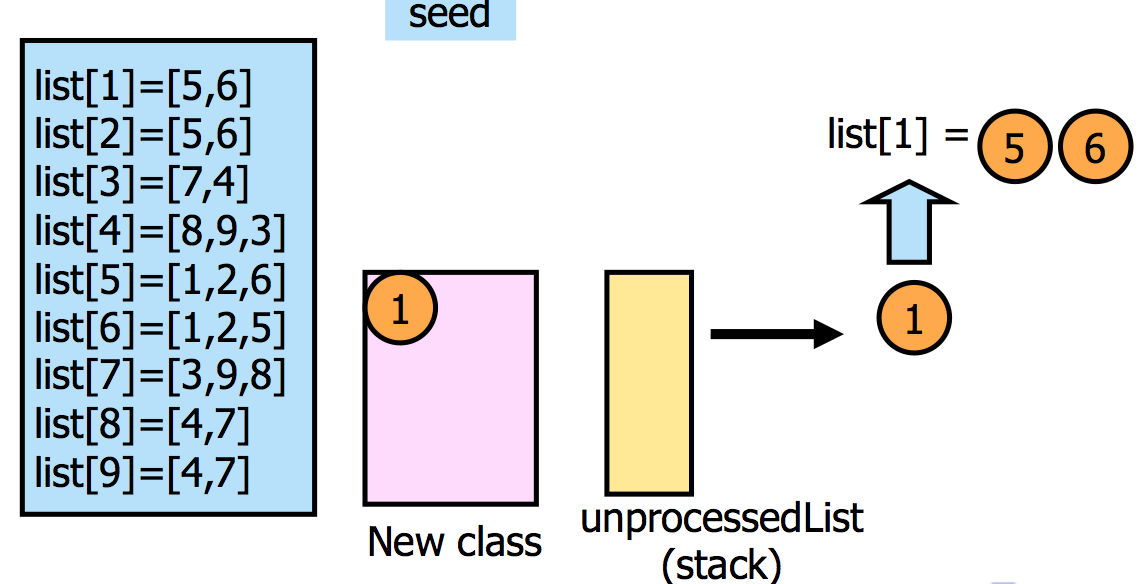
\includegraphics[scale=0.35]{pics/offline_2.png}  \newline
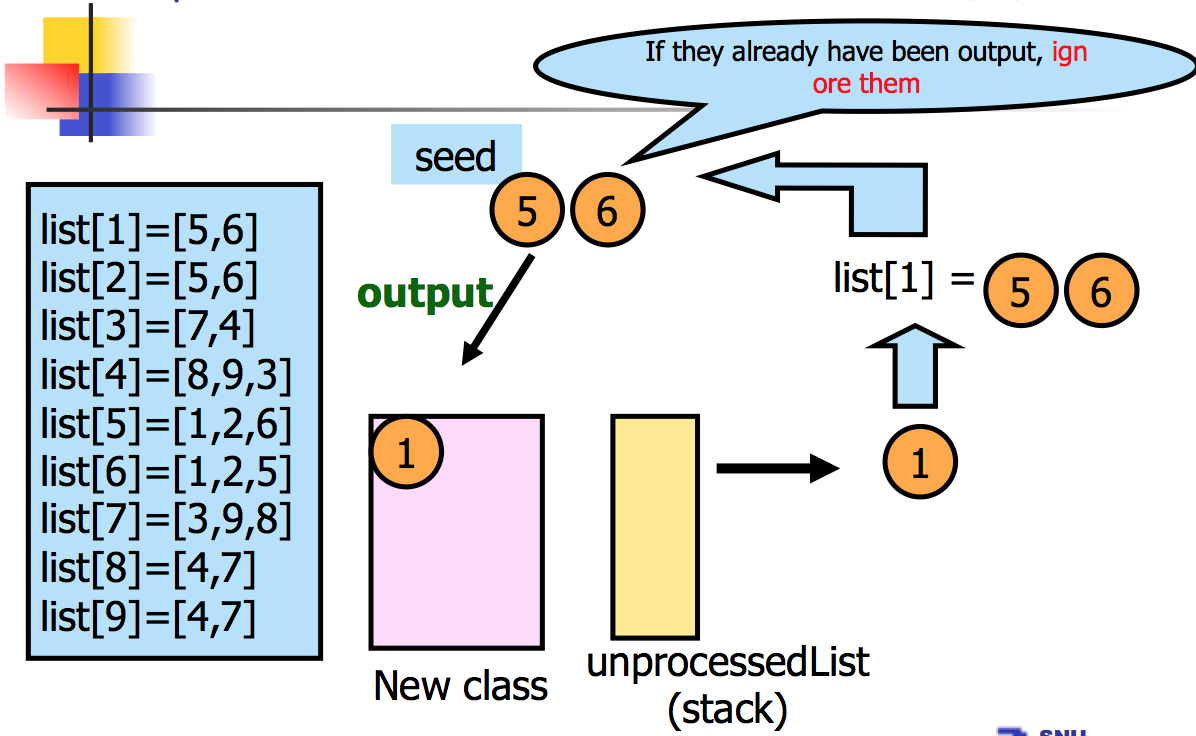
\includegraphics[scale=0.35]{pics/offline_3.png} \newline
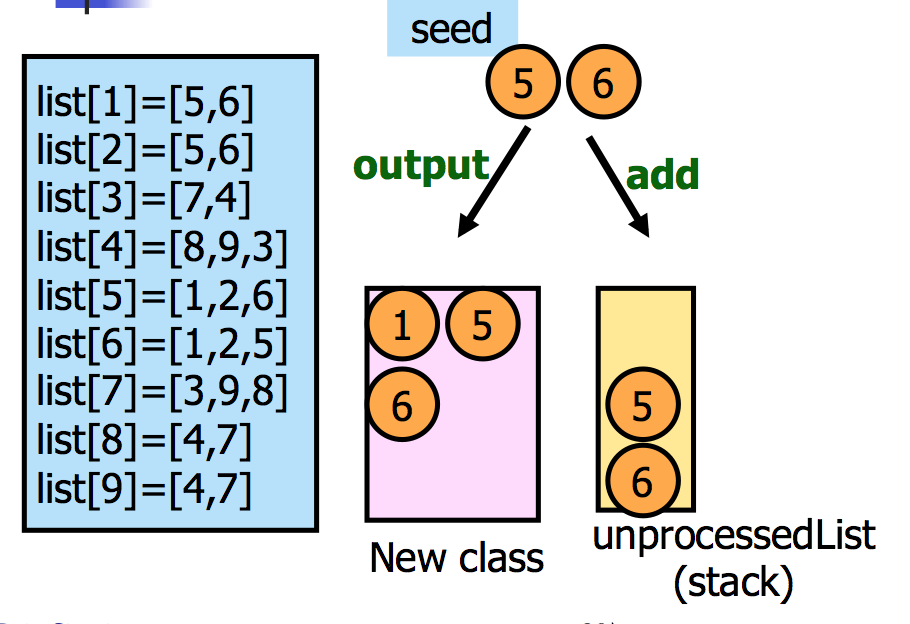
\includegraphics[scale=0.35]{pics/offline_4.png} \newline
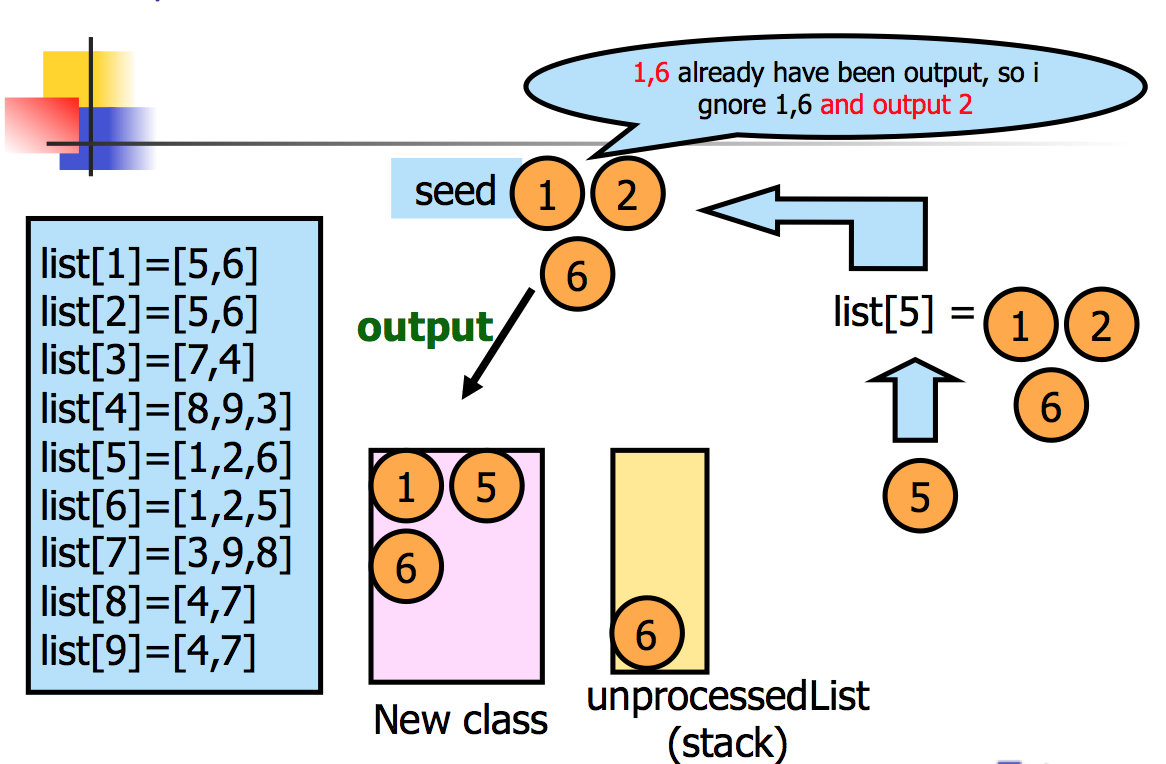
\includegraphics[scale=0.35]{pics/offline_5.png} \newline
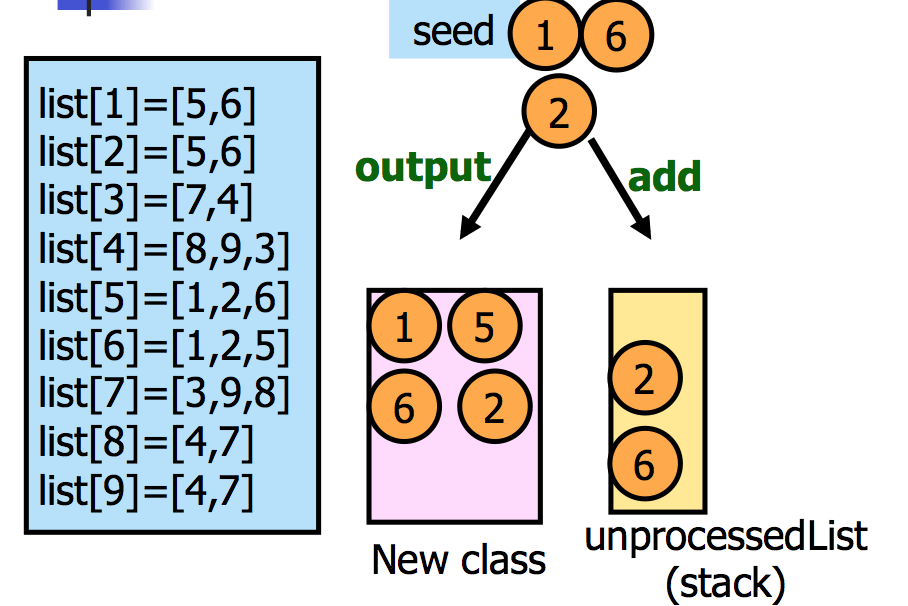
\includegraphics[scale=0.35]{pics/offline_6.png} \newline


\end{itemize}

\subsubsection{Other interview questions}
\begin{itemize}
\item How to Reverse a list \textbf{ There are two points: 1)while(p),  2) inside loop, do p = p->next, and necessary action( print out value and change pointer direction...)}
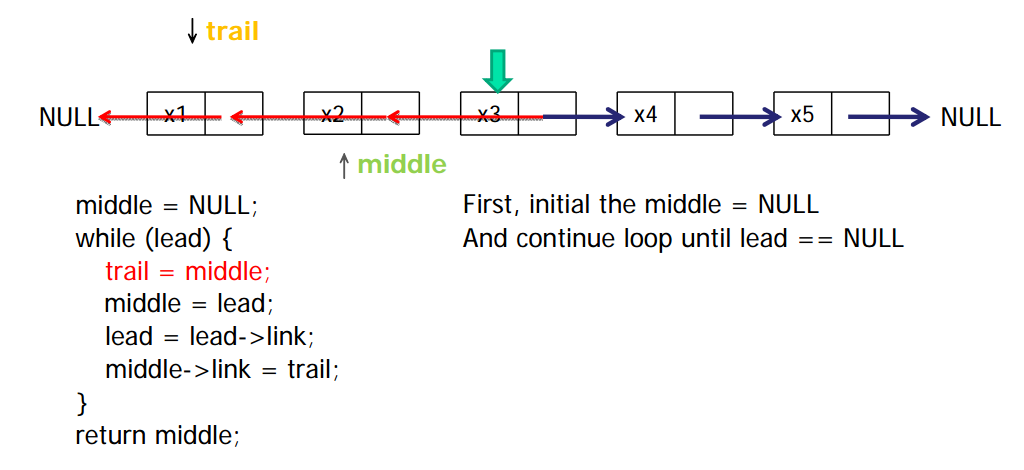
\includegraphics[scale=0.65]{pics/reverse.png} \newline


\begin{lstlisting}[breaklines]
node* lead; 
node *middle, *tail;
middle = nullptr;
tail = head;
while(tail){
	lead = middle;
	middle = tail;
	tail = tail->next;
	middle->next = lead;
}

head = middle;
\end{lstlisting}
\begin{description}
	\item[line] end condition
	\item[line] end-input condition
	\item[line] begin condition
	\item[line] begin-input condition
\end{description}
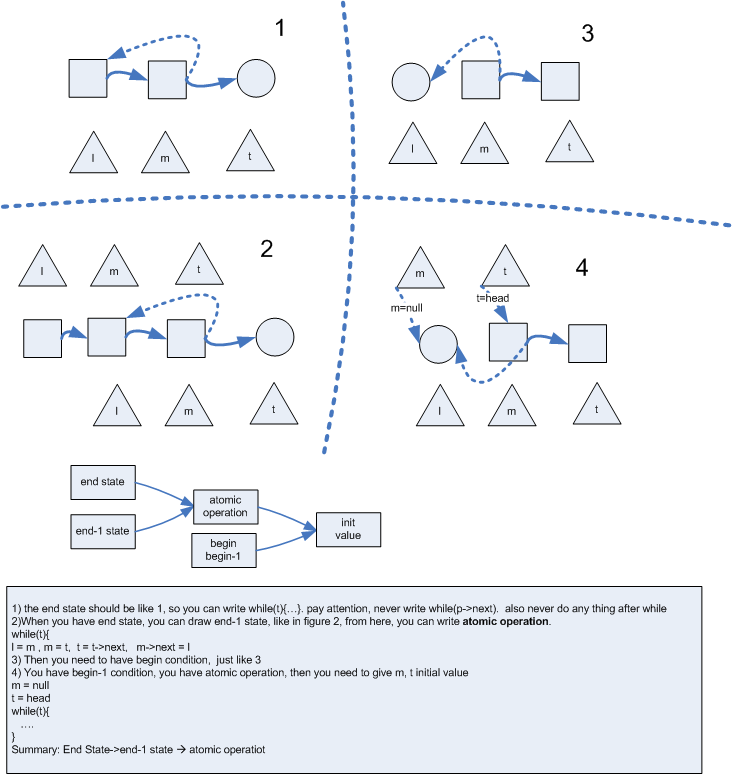
\includegraphics[scale=0.65]{pics/link.png} \newline

\item Find the middle of a given linked list: 
\begin{lstlisting}[breaklines]
Traverse linked list using two pointers. Move one pointer by one and other pointer by two. When the fast pointer reaches end slow pointer will reach middle of the linked list.
\end{lstlisting}
\textbf{Idea: Keep two pointer at the same time}

\item Given a singly linked list, determine if its a palindrome. This method takes O(n) time and O(1) extra space.
\begin{lstlisting}[breaklines]
1) Get the middle of the linked list.
2) Reverse the second half of the linked list.
3) Check if the first half and second half are identical.
4) Construct the original linked list by reversing the second half again and attaching it back to the first half.
\end{lstlisting}
\textbf{Idea: 1) find the middle 2)reverse}

\item Flatten A Binary Tree to Linked List (In-place) 
Go down through the left, when right is not null, push right to stack. \newline

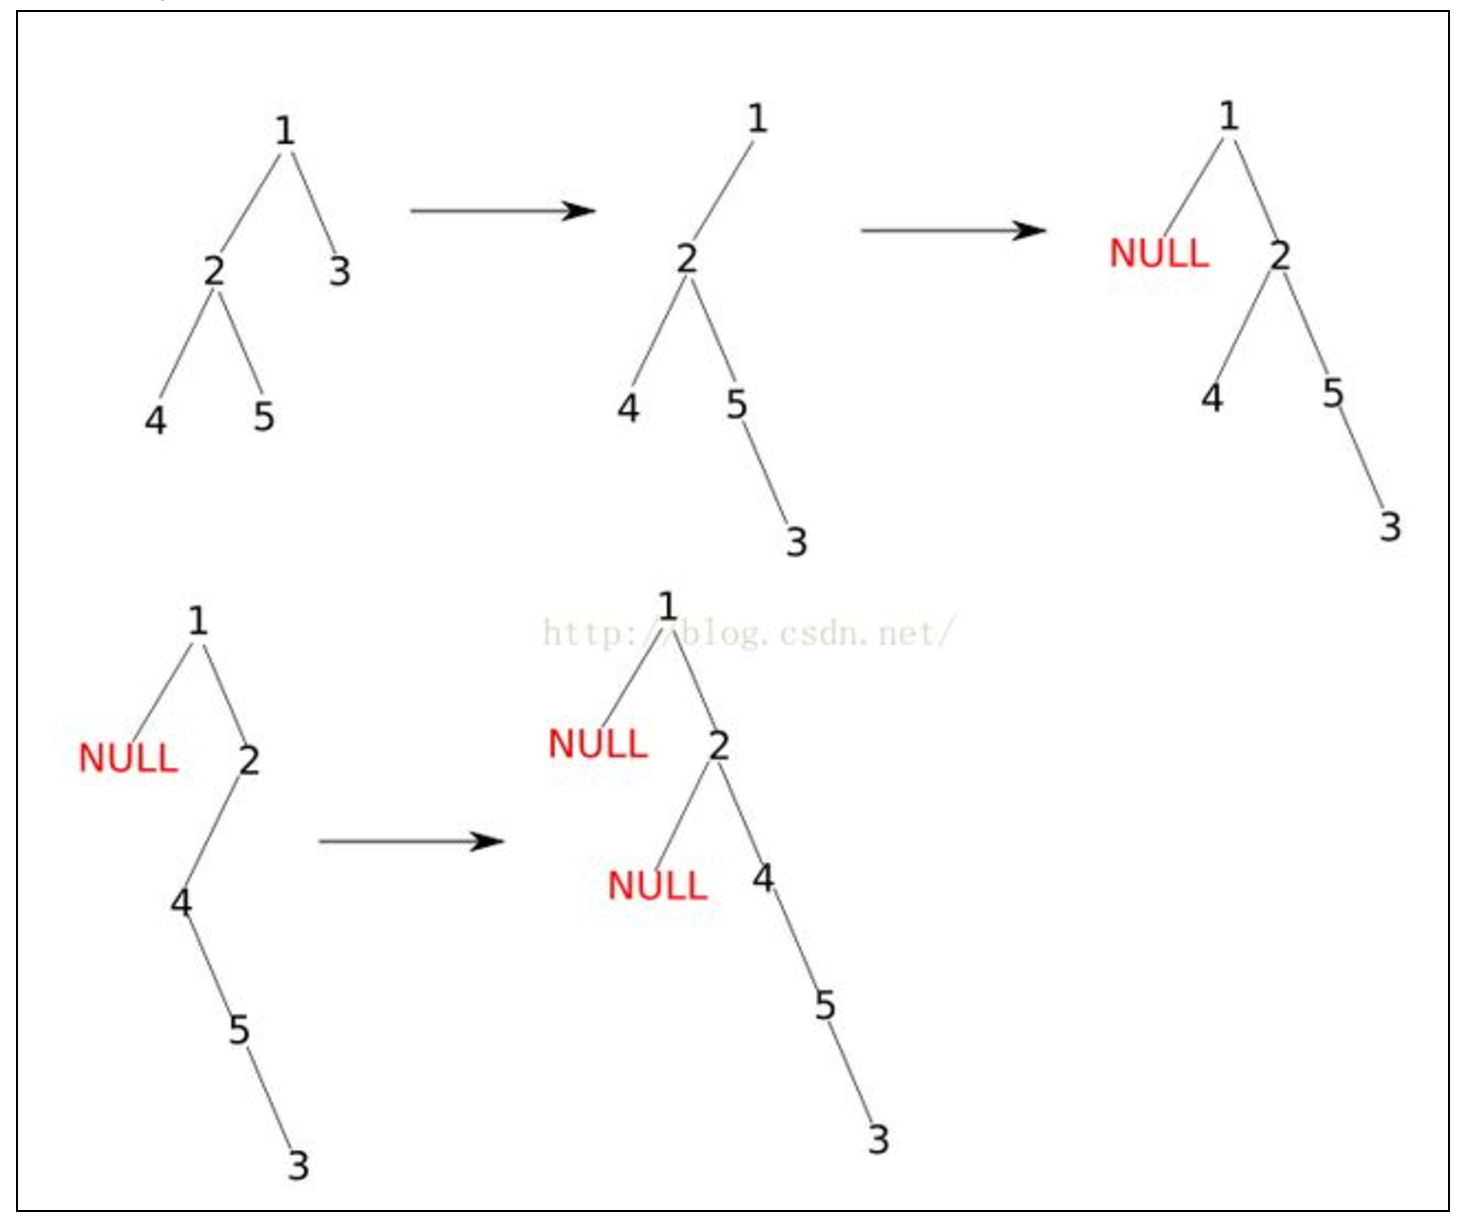
\includegraphics[scale=0.39]{pics/t2l.png} \newline
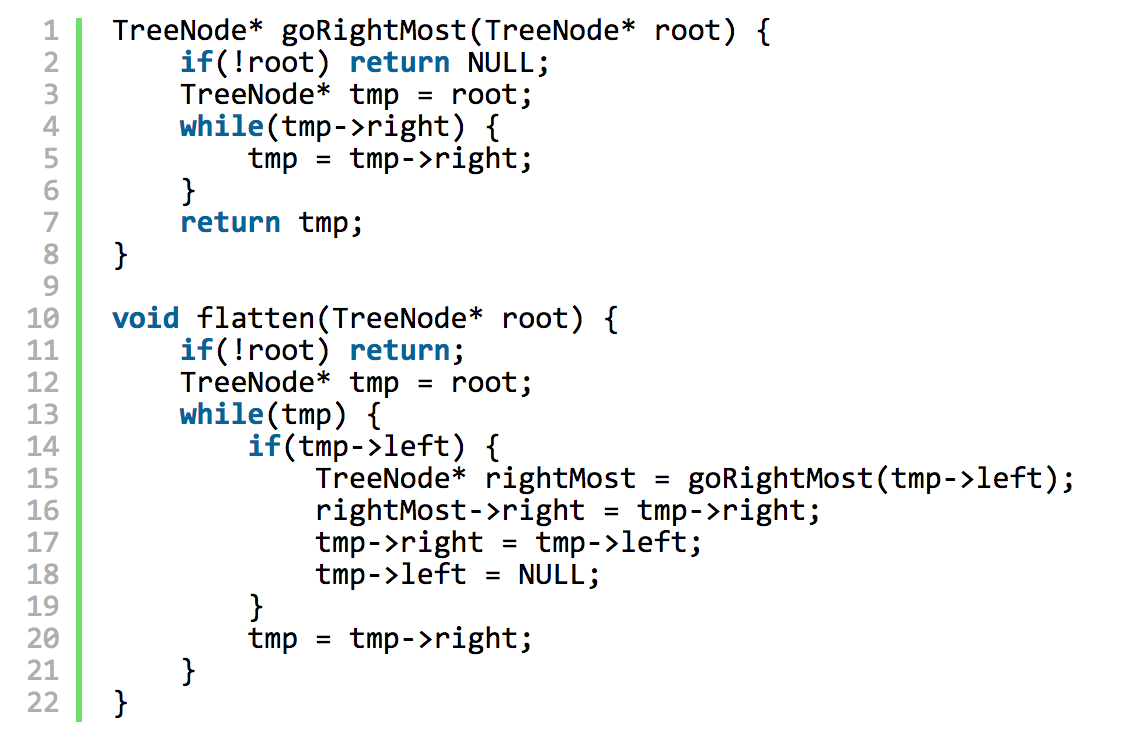
\includegraphics[scale=0.6]{pics/t2l1.png} \newline

\item Swap nodes in a linked list without swapping data. 
\begin{lstlisting}[breaklines]
The idea it to first search x and y in given linked list. If any of them is not present, then return. While searching for x and y, keep track of current and previous pointers.
\end{lstlisting}


\item Given only a pointer/reference to a node to be deleted in a singly linked list, how do you delete it?
\begin{lstlisting}[breaklines]
is to copy the data from the next node to the node to be deleted and delete the next node. Something like following.
\end{lstlisting}

\item Merge sort is often preferred for sorting a linked list. The slow random-access performance of a linked list makes some other algorithms (such as quicksort) perform poorly, and others (such as heapsort) completely impossible. MergeSort(headRef)
\begin{verbatim}
1) If head is NULL or there is only one element in the Linked List 
    then return.
2) Else divide the linked list into two halves.  
      FrontBackSplit(head, &a, &b); /* a and b are two halves */
3) Sort the two halves a and b.
      MergeSort(a);
      MergeSort(b);
4) Merge the sorted a and b (using SortedMerge() discussed here) 
   and update the head pointer using headRef.
     *headRef = SortedMerge(a, b);
\end{verbatim}
\textbf{Idea: 1) No random access 2) recursive}

\begin{lstlisting}[frame=single, language=c++] 
/* sorts the linked list by changing next pointers (not data) */
void MergeSort(struct node** headRef)
{
  struct node* head = *headRef;
  struct node* a, b;
 
  /* Base case -- length 0 or 1 */
  if ((head == NULL) || (head->next == NULL)){
    return;
  }

  /* Split head into 'a' and 'b' sublists */
  FrontBackSplit(head, &a, &b); 
 
  /* Recursively sort the sublists */
  MergeSort(&a);
  MergeSort(&b);
 
  /* answer = merge the two sorted lists together */
  *headRef = SortedMerge(a, b);
}

\end{lstlisting}

 \begin{lstlisting}[frame=single, language=c++] 
/* See http://geeksforgeeks.org/?p=3622 for details of this 
   function */
struct node* SortedMerge(struct node* a, struct node* b)
{
  struct node* result = NULL;
 
  /* Base cases */
  if (a == NULL)
     return(b);
  else if (b==NULL)
     return(a);
 
  /* Pick either a or b, and recur */
  if (a->data <= b->data){
     result = a;
     result->next = SortedMerge(a->next, b);
  }
  else{
     result = b;
     result->next = SortedMerge(a, b->next);
  }
  return(result);
}
 \end{lstlisting}
 
 \begin{lstlisting}[frame=single, language=c++] 
/* UTILITY FUNCTIONS */
/* Split the nodes of the given list into front and back halves,
     and return the two lists using the reference parameters.
     If the length is odd, the extra node should go in the front list.
     Uses the fast/slow pointer strategy.  */
void FrontBackSplit(struct node* source,
          struct node** frontRef, struct node** backRef)
{
  struct node* fast;
  struct node* slow;
  if (source==NULL || source->next==NULL)
  {
    /* length < 2 cases */
    *frontRef = source;
    *backRef = NULL;
  }
  else
  {
    slow = source;
    fast = source->next;
 
    /* Advance 'fast' two nodes, and advance 'slow' one node */
    while (fast != NULL)
    {
      fast = fast->next;
      if (fast != NULL)
      {
        slow = slow->next;
        fast = fast->next;
      }
    }
 
    /* 'slow' is before the midpoint in the list, so split it in two
      at that point. */
    *frontRef = source;
    *backRef = slow->next;
    slow->next = NULL;
  }
}

\end{lstlisting}

\item Merge Two sorted lists.
\begin{lstlisting}[frame=single, language=c++]
/* Takes two lists sorted in increasing order, and splices
   their nodes together to make one big sorted list which
   is returned.  */
struct node* SortedMerge(struct node* a, struct node* b){
    /* a dummy first node to hang the result on */
    struct node dummy;
    /* tail points to the last result node  */
    struct node* tail = &dummy;

    /* so tail->next is the place to add new nodes
      to the result. */
    dummy.next = NULL;
    while (1){
        if (a == NULL)        {
            /* if either list runs out, use the
               other list */
            tail->next = b;
            break;
        }
        else if (b == NULL){
            tail->next = a;
            break;
        }
        if (a->data <= b->data)
            MoveNode(&(tail->next), &a);
        else
            MoveNode(&(tail->next), &b);
 
        tail = tail->next;
    }
    return(dummy.next);
    //dummy code will be destoried. 
}
 \end{lstlisting}

\begin{lstlisting}[frame=single, language=c++] 
/* UTILITY FUNCTIONS */
/* MoveNode() function takes the node from the front of the
   source, and move it to the front of the dest.
   It is an error to call this with the source list empty.
   Before calling MoveNode():
   source == {1, 2, 3}  dest == {1, 2, 3}
   Affter calling MoveNode():
   source == {2, 3}  dest == {1, 1, 2, 3} */
void MoveNode(struct node** destRef, struct node** sourceRef)
{
    /* the front source node  */
    struct node* newNode = *sourceRef;
    assert(newNode != NULL);
 
    /* Advance the source pointer */
    *sourceRef = newNode->next;
 
    /* Link the old dest off the new node */
    newNode->next = *destRef;
 
    /* Move dest to point to the new node */
    *destRef = newNode;
}
\end{lstlisting}

\item fun1() prints the given Linked List in reverse manner. 
\begin{lstlisting}[frame=single, language=c++]
void fun1(struct node* head){
  if(head == NULL)
    return;
  
  fun1(head->next);
  printf("%d  ", head->data);
}
\end{lstlisting}
\textbf{Idea: recursive}



\item Write a program function to detect loop in a linked list
\begin{lstlisting}[breaklines]
This is the fastest method. Traverse linked list using two pointers.  Move one pointer by one and other pointer by two.  If these pointers meet at some node then there is a loop.  If pointers do not meet then linked list doesn't have loop.
\end{lstlisting}
\textbf{a circle has at last three nodes, so fast pointer each time step 2, So it will always go around inside the circle}

\item Conclusion:
\begin{enumerate}
\item Just like tree, link-list problems can be resolved by recursive. 
\item Most of time, In single link list, you need to keep previous pointer. 
\end{enumerate}

\begin{tabular}{|c|c|c|}
\hline 
 & array & list \\ 
\hline 
insert erase & O(n) & O(1) \\ 
\hline 
sort & quicksort & mergesort  \\ 
\hline 
reverse & swap element & just manipulate pointer  \\ 
\hline 
rotate & easy pointer manipulate & swap element  \\ 
\hline 
merge &  &  \\ 
\hline 
other  &  &  \\ 
\hline 

\end{tabular} 

\begin{enumerate}
\item in STL,  For assign, insert, erase and constructor, vector support two version, one is single element, other is range.  When we deal wih range input, we prefer to use range version. 
\item std::list and std::vector has different big O for insert and erase.
\item std::list has its own sort member function, but std::vector doesn't have. you can use std::sort algorithme. 
\item std::list has its own reverse,  std::vector doesn't have, just use std::reverse algorithm
\item list and vector don't have their own rotate function.
\item list has its own merge, vector use std::merge algorithm.

\end{enumerate}







\end{itemize}
\section{Matrix}
\begin{itemize}
\item You can use two dimensions array to act as a matrix, square matrix, diagonal matrix, lower triangular, symmetric. 
\item Some special square matrix
\begin{enumerate}
\item Diagonal  $i\neq j, M(i,j) = 0$ Can use one dimension array to describe it. 
\item Low triangular $i<j, M(i,j) = 0$ We can use one dimension array to implement lower triangular because it will save many spaces.  Index can be calculated by $i*(i-1)/2+j-1$. and save it into a one dimension array. 
\item Symmetric. Just like Low triangular, can be descriped by one dimenstion array. 
\end{enumerate}
\end{itemize}

\subsubsection{sparse matrix}
\begin{itemize}
\item Sparse matrix can implemented by on dimension array or  linked list. 
\begin{lstlisting}[frame=single, language=c++]
template<typename T>
class term{
int row, int col;
T value;
}

Term<T> *sparseMatrix;
\end{lstlisting}

\item Sparse matrix in linked list.  \textbf{Three level definition}
\begin{lstlisting}[frame=single, language=c++]
template<typenameT>
class CNode{
int col;
T value;
};

template<typename T>
class HeadNode{
int row, 
Chain< CNode<T> > colFirst
};
  
template<typename T>
class Matrix{
  Chain< HeadNode<T> > Frist
} 
\end{lstlisting}


\item You can build a matrix class. use m(2,3) to access a element. And support +, - * . You also can define index begin from 1. It will more reasonable for you when you use a matrix. 
\begin{lstlisting}[frame=single, language=c++]
template<typename T>
class Matrix{
T& operator()(int row, int col){
..}
}
\end{lstlisting} 

\end{itemize}

 
\section{Stack}
\begin{itemize}
\item In C++ STL , stack<template> is container adaptor, specifically designed to operate in a LIFO context. In C\#: Stack myStack = new Stack();

\item Stack is last-in first-out, and queue is frist-in and first-out

\end{itemize}
\subsection{Application of Stack}
\begin{itemize}
\item The most famous application about stack is \textbf{Recursive}.
\item \textbf{The most famous applications based on stack is:  Maze(depth first). Hanoi tower. brace Match, recursive.}  

\item Next Greater Element.  Given an array, print the Next Greater Element (NGE) for every element. The Next greater Element for an element x is the first greater element on the right side of x in array. Elements for which no greater element exist, consider next greater element as -1.
\begin{verbatim}
Examples:
a) For any array, rightmost element always has next greater element as -1.
b) For an array which is sorted in decreasing order, all elements have next greater element as -1.
c) For the input array [4, 5, 2, 25}, the next greater elements for each element are as follows.
Element       NGE
   4      -->   5
   5      -->   25
   2      -->   25
   25     -->   -1
\end{verbatim}

\begin{lstlisting}[breaklines]
1) Push the first element to stack.
2) Pick rest of the elements one by one and follow following steps in loop.
...a) Mark the current element as next.
...b) If stack is not empty, then pop an element from stack and compare it with next.
...c) If next is greater than the popped element, then next is the next greater element for the popped element.
...d) Keep popping from the stack while the popped element is smaller than next. next becomes the next greater element for all such popped elements
...g) If next is smaller than the popped element, then push the popped element back.
3) After the loop in step 2 is over, pop all the elements from stack and print -1 as next element for them.
\end{lstlisting}

\end{itemize}


\section{Queue}
\begin{itemize}
\item In STL, Queue has front() and back() interface. 

\end{itemize}

\subsection{Circule Queue}
\begin{itemize}
\item circular array representation of a queue
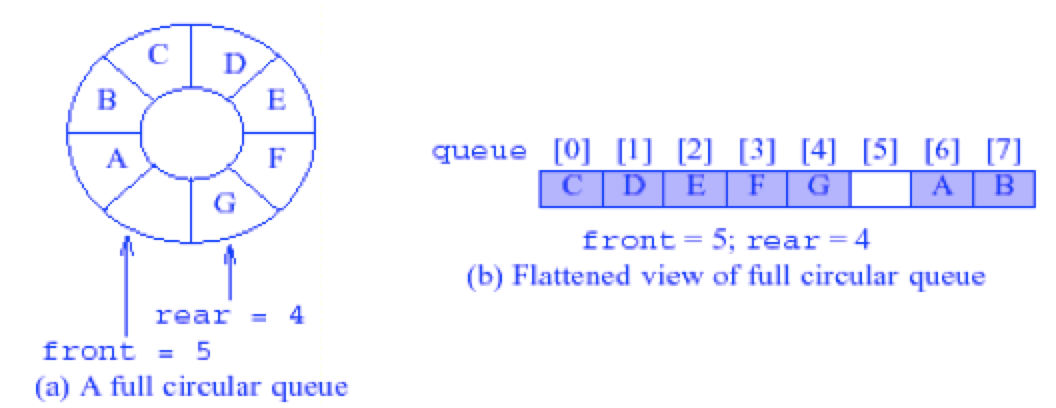
\includegraphics[scale=0.35]{pics/cd.png} \newline
\begin{enumerate}
\item Initial condition : front = rear = 0
\item Empty queue:     front --> rear
\item Full: (rear+1)\%length --> front
\item front point to an empty cell. So at mast it can save length-1 elements. 
\item push only increase rear, so if (rear+1)\%length --> front, means rear catch up front, it means full. 
\item pop only increase front, so if front --> rear, means front catch up rear, it means empty.
\end{enumerate}
\end{itemize}


\subsection{Application of queue}
\begin{itemize}
\item  BFS maze 
\begin{lstlisting}[frame=single, language=c++]
here=root of T;
here is end?
enqueue(Q,v);

while(!empty(Q)){
    dequeue(Q, here);
    if(here is end)
    for (each next position of here){
        if(next position is not end){
             mark next position
             enqueue(Q, next position);
        }
    }
}
\end{lstlisting}

\item For BFS, path is not save in stack. So you need a new kind of data type. 
\begin{lstlisting}[frame=single, language=c++]
struct position {
        int x;
        int y;
        struct position* parent;
}
\end{lstlisting}
\item Just like DFS, before you add a position to queue, mark it first. 

\end{itemize}

\section{Heap}

\begin{itemize}
\item Max(min) tree is each node is greater or equal to its children node.
\item Heap is \textbf{1)complete 2) binary 3)Max(min) tree.}
\item Because Heap is complete binary tree. We can use an array to store it. 
\item insert is easier than you think, When you insert, put it on the end position, then exchange with parent.  


\begin{lstlisting}[frame=single, language=c++, mathescape=true]
vector<int> vi = {2, 4, 1, 3, 5,6,7};
cout<<"ddd"<<distance(end(vi),begin(vi))<<endl;
make_heap(begin(vi),end(vi)); // inpace modify

//after you pop_heap, you need to use v.pop_back()
//to make begin(vi), end(vi) is still heap. 
v.pop_heap(begin(vi),end(vi));
v.pop_back();

//if you want to use push_heap, you have to 
//call push_back first. 
v.push_back(10);
v.push_heap(v.begin(vi) ,end(vi));

//still inpace modify
sort_heap(v.begin(vi) ,end(vi));
\end{lstlisting}



\begin{lstlisting}[frame=single, language=c++, mathescape=true]
insert(x){
  int c = ++currentSize;
  while(c!=1 && x>heap[c/2]){ //get its parent node and compare
  heap[c] = heap[c/2];  //move down parent
  $\Hilight{20}$// move parent  down because it smaller
  c/=2;  //move up a level 
  }  
  heap[c] = x;  //the right position of insert. 
  //at this time heap[c] has been moved away by previous 
  //statement heap[c] = heap[c/2] 
}
$\Hilight{20}$ //c is used to control level,  c/=2 move up level
$\Hilight{20}$ //heap[c/2] get its parent
\end{lstlisting}

\item \textbf{Heap just support delete Max(Min) value.} When delete, delete the first element, then put the end position element to the first position, then exchange it with either left child or right child. 
\begin{lstlisting}[frame=single, language=c++, mathescape=true]
T y = heap[CurrentSize--];
int i = 1, ci = 2;
//because ci will increase to get bigger one from two children.
//so I have to use another i to keep current level
while(ci<=CurrentSize){
  if(heap[ci]<heap[ci+1]) ci++; // get the bigger child
  
  if(y>=heap[ci]{
   heap[i] = y;   // i always empty for a new value. 
   break; 
  }
  $\Hilight{10}$ //i is current node
      $\Hilight{10}$ //ci  is i biggest child node
  heap[i] = heap[ci]; //move up child, insert is "move down parent"
  i = ci;  //move to next level
  ci *=2;
}
\end{lstlisting}
\item Initialize a Heap: \textbf{For an array, from the middle point, loop backward until reach  head}. the time complexity is O(n). 

\begin{lstlisting}[frame=single, language=c++]
for(int i = CurrentSize/2; i>=1;i--){ //from middle, backward
 root = head[i] // get root node
 child1 = root*2, child2 = root*2+1 // get two children
 move bigger child to root.
}
\end{lstlisting}

\item Heap just guarantees that elements on higher levels are greater (for max-heap) or smaller (for min-heap) than elements on lower levels, whereas BST guarantees order (from "left" to "right"). If you want sorted elements, go with BST.

\item In STL, heap is called priority\_queue

\begin{lstlisting}[frame=single, language=c++, mathescape=true]
$\Hilight{15} default compare function is less<T>$
 std::priority_queue<int, std::vector<int>, std::greater<int> > q2;
    for(int n : {1,8,5,6,3,4,0,9,7,2})
        q2.push(n);
    // 0, 1, 2 ,3 ,4, 5...
\end{lstlisting}

\end{itemize}


\subsubsection{application}
\begin{itemize}
\item \textbf{Huffman tree use external nodes to represent a character, It assure no prefix is repeated }
\item You can use minHeap to build huffman tree. in the minHeap, each element is child tree, and then pop twice, combine two child trees. then insert it back to minHeap. Until there is only one element in the Heap. 
\end{itemize}

\section{Tree}
\begin{itemize}
\item List has a first node, every tree has a root node. 

\item Pre-order, In-order and Post-order are based on middle node. \textbf{and they are all dfs algorithm.}

\item Balance search tree includes AVL and RB tree, in order to keep it balance, you need to rotate child tree. 

\item Tournament Tree: Tournament tree is a complete binary tree with some properties
Remove and  Replay of Tournament tree gives you "sorting".

\item Binary Search Tree: BST is a binary tree with some properties (not necessarily CBT)
In-order traversal of BST gives you "sorting" Can be skewed and unbalanced, so we need Balanaced Tree.

\end{itemize}
 
\subsection{Search Tree}
\begin{itemize}
\item Search tree is the key in each node must be \textbf{greater than all keys stored in the left sub-tree, and smaller than all keys in the right sub-tree.} 

\item Difference between BST and hash
\begin{enumerate}
\item So Hash Table seems to beating BST in all common operations. When should we prefer BST over Hash Tables, what are advantages. Following are some important points in favor of BSTs.

\item We can get all keys in sorted order by just doing Inorder Traversal of BST. This is not a natural operation in Hash Tables and requires extra efforts.

\item Doing order statistics, finding closest lower and greater elements, doing range queries are easy to do with BSTs. Like sorting, these operations are not a natural operation with Hash Tables.

\item BSTs are easy to implement compared to hashing, we can easily implement our own customized BST. To implement Hashing, we generally rely on libraries provided by programming languages.

\item With BSTs, all operations are guaranteed to work in O(Log(n) ) time. But with Hashing, O(1) is average time and some particular operations may be costly, especially when table resizing happens.
\end{enumerate}

\item ascending or descending order of BST
\begin{lstlisting}[frame=single, language=c++]
void ascending(BST* root){
    if(root == NULL) return;
    ascending(root->left);
    std::cout<<root->data<<" ";
    ascending(root->right);
}
 
void descending(BST* root){
    if(root == NULL) return;
    descending(root->right);
    std::cout<<root->data<<" ";
    descending(root->left);
}
\end{lstlisting}

\end{itemize}


\subsection{Tree and recursion} 
\textbf{Nearly all the tree problems can be resolved by recursive}. When you recursive tree traversal,  There are some points that you need to pay attention to:
\begin{enumerate}
\item \textbf{Forgetting to check if the root is null. It's an important base case.}

\item \textbf{Checking if one or both children are null. You SHOULD NOT do that.} When you do the recursive call and pass the root.left() or the root.right() as the parameter, the recursive function will call itself and treating the passed child as the new root. So, you don't need to explicitly check if the children are null.

\item \textbf{Accessing the children values. You SHOULD NOT do that.} The same as the previous point. The child passed to the recursive call is treated as the new root. So, you don't need to explicitly access the children values. Just make sure you do that for the root.

\item If it is required from you to write a function that returns a value (e.g. the number of nodes in a binary tree), you have to make sure that the function actually "returns". One of the common mistakes is just writing the recursive call without writing the word "return" before it.

 \item If you write a recursive tree  that returns a value, the left and right branching should be done in an assignment statement, e.g.,
\begin{lstlisting}[frame=single, language=c++]
private int height(Node t){
     if(t == null)  {  //1) base case
        return -1;   //5) return value 
     }
     else
     {
         int height = 1 + max( height(t.left), height(t.right) );
         //5) put left and right recursive into assignment
         return height;
     }
}
\end{lstlisting}

\begin{lstlisting}[frame=single, language=c++]
private int countLeaves(Node t){
   if(t == null) 
         return 0;
         
         if(isLeaf(t))  {
             return 1;
         }
         else
             return countLeaves(t.left) +countLeaves( t.right);
     }
    
\end{lstlisting}

\item how many nodes are there in a tree. 
\begin{lstlisting}[frame=single, language=c++]
int BinaryTree::size(Node *leaf) const {
    if(leaf == NULL) { //This node doesn't exist. Therefore there are no nodes in this 'subtree'
        return 0;
    } else { //Add the size of the left and right trees, then add 1 (which is the current node)
        return size(leaf->getLeft()) + size(leaf->getRight()) + 1;
    }
}
\end{lstlisting}

\item Information flow:
 \begin{enumerate}
\item  return value from child to parent, (only return one value, so need some calculation inside from both left and right children)
\item pass from parent to child, parameter to remember auto value(level) , 
\item shared between children and parent. and pass a pointer parameter(max\_level) to remember static, which all recursive 
 \end{enumerate}
 
\begin{lstlisting}[frame=single, language=c++]
// Recursive function to print left view of a binary tree.
void leftViewUtil(struct node *root, int level, int *max_level){
    // Base Case
    if (root==NULL)  return;
 
    // If this is the first node of its level
    if (*max_level < level){
        printf("%d\t", root->data);
        *max_level = level;
    }
    
    // Recur for left and right subtrees
    leftViewUtil(root->left, level+1, max_level);
    leftViewUtil(root->right, level+1, max_level);
}
 \end{lstlisting}

\item recursive can be used to deal with two trees at the same time. 
\begin{lstlisting}[frame=single, language=c++]
int identicalTrees(struct node* a, struct node* b){
    /*1. both empty */
    if (a==NULL && b==NULL)
        return 1;
         
    /* 2. both non-empty -> compare them */
    if (a!=NULL && b!=NULL)    {
        return(
            a->data == b->data &&
            identicalTrees(a->left, b->left) &&
            identicalTrees(a->right, b->right)
        );
    } 
        
    /* 3. one empty, one not -> false */
    return 0;
} 
\end{lstlisting}


\end{enumerate}

Conclusion:
\begin{enumerate}
\item According to question, if it will return a value, such as leaf count, height. It has to have a function. 
\item Write base case 
\begin{lstlisting}[breaklines]
if(root == nullptr) 
       return [value] 
\end{lstlisting}
\item consider a node with two null children. that is the easiest tree. then finish the basic logic. At this time. value of function on left and right children have been known by the previous base case
\begin{lstlisting}[breaklines]
// If this is calculate how many nodes.
if(root == nullptr) 
       return 0;
     return 1+ recursive(root->left) + recursive(root-right);
     //so a node tree, nodeNum(root->left) return 0. 
     
     cout<<node<<endl;
     recursive(root->left);
     recursive(root->right);     
     //or print a node.  such as pre-order, in-order, post-order traversal. 
\end{lstlisting}

\item For some easy problems, you have finished the problems. Then for some difficult problems, you need to some logic comparison or calculation. such as Maximum path sum in a binary tree. or max height tree.



\end{enumerate}

\subsection{Application}
\begin{itemize}
\item Maximum Path Sum in a Binary Tree. 
\begin{lstlisting}[breaklines]
For each node there can be four ways that the max path goes through the node:
1. Node only
2. Max path through Left Child + Node
3. Max path through Right Child + Node
4. Max path through Left Child + Node + Max path through Right Child

The idea is to keep trace of four paths and pick up the max one in the end. An important thing to note is, root of every subtree need to return maximum path sum such that at most one child of root is involved. This is needed for parent function call. In below code, this sum is stored in 'max_single' and returned by the recursive function.
\end{lstlisting}

\textbf{Idea: (recursive + return style)}

\item in order without recursive, 
\begin{lstlisting}[frame=single, language=c++]
// An iterative process to print preorder traversal of Binary tree
void iterativePreorder(node *root){
    // Base Case
    if (root == NULL)
       return;
 
    // Create an empty stack and push root to it
    stack<node *> nodeStack;
    nodeStack.push(root);
 
    /* Pop all items one by one. Do following for every popped item
       a) print it
       b) push its right child
       c) push its left child
    Note that right child is pushed first so that left is processed first */
    while (nodeStack.empty() == false)    {
        // Pop the top item from stack and print it
        struct node *node = nodeStack.top();
        printf ("%d ", node->data);
        nodeStack.pop();
 
        // Push right and left children of the popped node to stack
        if (node->right)
            nodeStack.push(node->right);
        if (node->left)
            nodeStack.push(node->left);
    }
}
\end{lstlisting}

\textbf{Idea: A common implementation of DFS, without check two unvisited condition. Because tree is a 1) minimally connected graph and having only one path between any two vertices. 2) no loop}

\item For search tree, look for lowest common ancestor(LCA). 
\begin{lstlisting}[frame=single, language=c++]
Node *LCA(Node *root, Node *p, Node *q) {
  if (!root || !p || !q) return NULL;
  if (max(p->data, q->data) < root->data)
    return LCA(root->left, p, q);
  else if (min(p->data, q->data) > root->data)
    return LCA(root->right, p, q);
  else
    return root;
}

\end{lstlisting}

\item Find a LCA in any tree. 

\begin{lstlisting}[frame=single, language=c++]
Method 1 (By Storing root to n1 and root to n2 paths):
Following is simple O(n) algorithm to find LCA of n1 and n2.
1) Find path from root to n1 and store it in a vector or array.
2) Find path from root to n2 and store it in another vector or array.
3) Traverse both paths till the values in arrays are same. Return the common element just before the mismatch.
\end{lstlisting}

\item  If target is present in tree, then prints all the ancestors and returns true, otherwise returns false. 
\begin{verbatim}
              1
            /   \
          2      3
        /  \
      4     5
     /
    7
 key is 7, then your function should print 4, 2 and 1.
\end{verbatim}

\begin{lstlisting}[frame=single, language=c++]
bool printAncestors(struct node *root, int target){
  /* base cases */
  if (root == NULL)
     return false;
  if (root->data == target)
     return true;
     
  /* If target is present in either left or right subtree of this node,
     then print this node */
  if ( printAncestors(root->left, target) ||
       printAncestors(root->right, target) ){
    cout << root->data << " ";
    return true;
  }
  /* Else return false */
  return false;
}
\end{lstlisting}
\textbf{Idea: just like max height example, return bool instead value, logic || instead max. the basic idea are quite same. }

\end{itemize}



        \section{Graph}
\subsection{Basic}
\begin{itemize}
\item \textbf{A Tree is just a restricted form of a Graph. They fit with in the category of Directed Acyclic Graphs (or a DAG). So Trees are DAGs with the restriction that a child can only have one parent.}

\item Graphs are generally search breath first or depth first. The same applies to Tree.

\item Basic represent way: adjacency list and adjacency matrix: \newline
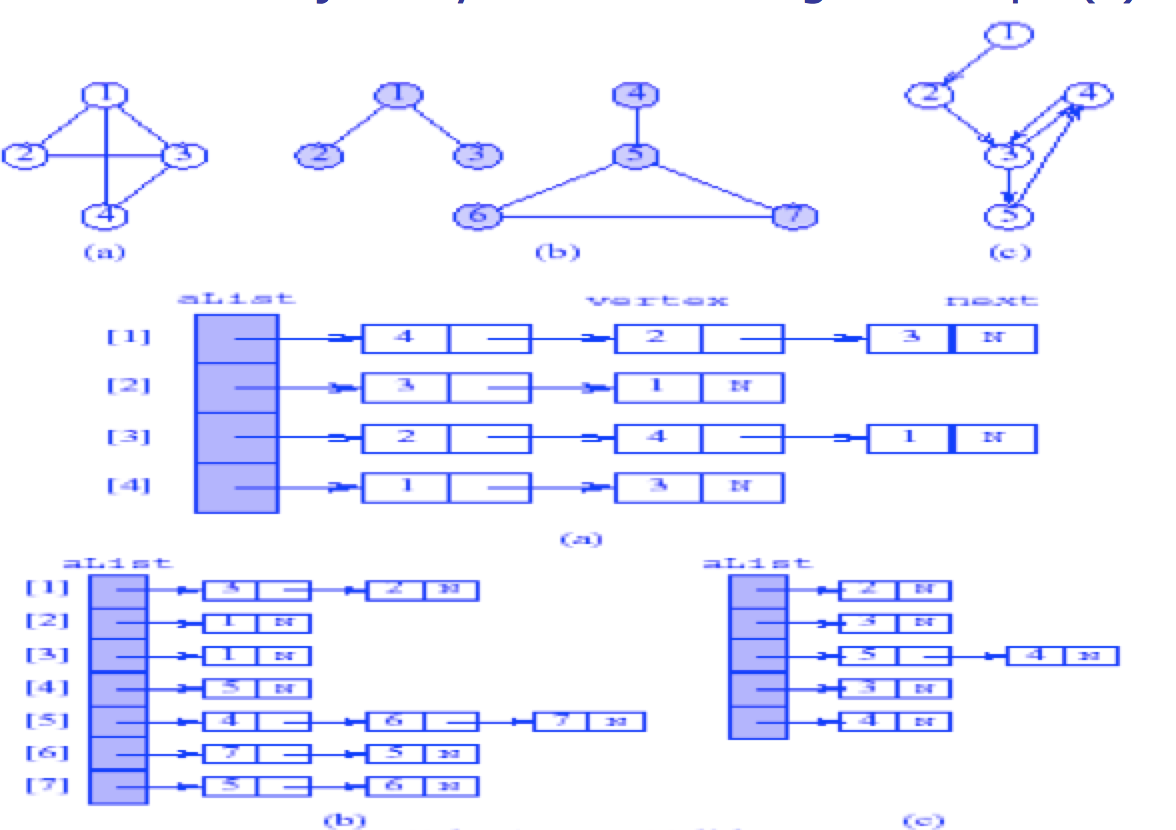
\includegraphics[scale=0.6]{pics/adjacency.png} \newline

\item You want to mirror the problem using a tree-like structure:For this we have boost graph library. The BGL currently provides two graph classes and an edge list adaptor: adjacency\_list, adjacency\_matrix and edge\_list.  The adjacency\_list class is the general purpose `"swiss army knife'' of graph classes.
\end{itemize}

\subsection{DFS and BFS}
\subsubsection{DFS}
\begin{itemize}
\item DFS has three versions 1) recursive 2) recursive to loop version. 3) uniform version
\begin{enumerate}
\item recursive version:
\begin{lstlisting}[frame=single, language=c++]
DFS(current){
  visit current;
  for all(next to current){
     if(unvisited(next)){
          DFS(next);
      }
   }
}
\end{lstlisting} 
\item recursive to loop
\begin{lstlisting}[frame=single, language=c++]
DFS(start){
 S.push(start)  
  while(!S.empty()){
    current = top();
    visit current;
    If (current has one unvisited next){ 
         stack.push(next);
    }   
    else{
        stack.pop()
    }
}
}
\end{lstlisting} 
\item unified version:
\begin{lstlisting}[frame=single, language=c++]
DFS(start){
 S.push(start)  
  while(!S.empty()){
    current = S.pop
    if(unvisited(current){
          visit current.
          for all(next to current and unvisited)
             S.push(next);
    }
  }
 }
\end{lstlisting} 
\end{enumerate}

\item  Why we need two "unvisited" words in DFS unified version.  
\begin{enumerate}
\item When we pop node from S, then we visit it, then we add all adjacent nodes to S, In this way, When we pop 1 from S, we add 2, 3 to S. at this time, 3 is unvisited, then when we pop 2 from S, we will add 4, 3 to S. so there are two 3 in the S. 
\item Based on, we need to first unvisit to avoid visit 3 twice

\item When we reach 3; 1,2,4 have been visited, so when we want to add all 3 adjacent, we need second unvisited to avoid 1,2,4 to S.  
\end{enumerate}
\begin{verbatim}
     1
  /    \
 2----3
 \     /
    4      
\end{verbatim}

\item DFS is an algorithm to search a hierarchical structure. But, pre-order traversal seems to be something similar also. So, what is the difference between the two?? DFS says:
\begin{enumerate}
\item If element found at root, return success.
\item If root has no descendants, return failure
\item Recursive DFS on left subtree: success if element found
\item If not, Recursive DFS on right subtree: success if element found
\end{enumerate}
Pre-order Traversal says:
\begin{enumerate}
\item Visit the root
\item Recursive pre-order on left subtree
\item Recursive pre-order on right subtree
\end{enumerate}

\end{itemize}

\subsubsection{BFS}

\begin{itemize}
\item There are two version of BFS:
\begin{enumerate}
\item Form DFS unify version, We can change S(stack) to Q(queue) and get unified version. \textbf{That is why we call it unified version}
\begin{lstlisting}[frame=single, language=c++]
BFS(start){
 Q.push(start)  
  while(!Q.empty()){
    current = Q.pop
    if(unvisited(current){
          visit current.
          for all(next to current and unvisited)
             Q.push(next);
    }
  }
 }
\end{lstlisting} 
\item Common version:  Unified version will have multi-copy vertex in the queue. We can improve it as below:  1) when you add it to queue, visit it. In this way, avoid add multi-copy vertex in queue 2) Because All the vertex in queue is visited, when you pop it, you don't need to judge if it's visisted. 
\begin{lstlisting}[frame=single, language=c++]
DFS(start){
 D.push(start)  
  while(!D.empty()){
    current = D.pop  //2) no if here
    for all(next to current and unvisited){
         visit current.  //1) push and visit at the same time. 
         D.push(next);
     }
  }
 }
\end{lstlisting} 

\item conclusion:
\begin{enumerate}
\item  \textbf{Conclusion, just remember unified version. 1) pop current, push neighbor, 2) check two unvisited}
\item unified version will push two nodes into stack or queue, so for BFS, you can visit and push at the same time, in this way, you don't need to check current if it is unvisited. 

\item For DFS, you can't use this way, because you can only visit only one neighbor, or it will become BFS. so each time, you just push one node into stack. It leads to two other versions. recursive version, and loop version. 
\end{enumerate}


\end{enumerate}

\item Path is saved in the stack.  when you quit while loop. just pop up each position from stack, then you get a path. But for BFS, you need extra information to save parent information. 
\end{itemize}

\subsection{spanning tree}
\begin{itemize}
\item 	BFS and DFS will produce spanning tree. 
\item The minimum spanning tree can be obtained in polynomial time:
\begin{enumerate}
\item Kruskal's algorithm
\item Prim's algorithm
\item Sollin's algorithm
\end{enumerate}

\item Kruskal algorithm:
\begin{lstlisting}[frame=single, language=c++]
KRUSKAL(G):
 A = empty
 foreach v in G.V:
    MAKE-SET(v)
 foreach (u, v) ordered by weight(u, v), increasing:
    if FIND-SET(u) != FIND-SET(v):
       A = A  {(u, v)}
       UNION(u, v)
 return A
\end{lstlisting}

\end{itemize}


\subsection{Application}
\begin{itemize}
\item detect a cycle in the graph
\begin{lstlisting}[frame=single, language=c++]
// A recursive function that uses visited[] and parent to detect
// cycle in subgraph reachable from vertex v.
bool Graph::isCyclicUtil(int v, bool visited[], int parent){
    // Mark the current node as visited
    visited[v] = true;
 
    // Recur for all the vertices adjacent to this vertex
    list<int>::iterator i;
    for (i = adj[v].begin(); i != adj[v].end(); ++i){
        // If an adjacent is not visited, then recur for that adjacent
        if (!visited[*i])        {
           if (isCyclicUtil(*i, visited, v))
              return true;
        }
        // If an adjacent is visited and not parent of current vertex,
        // then there is a cycle.
        else if (*i != parent)
           return true;
    }
    return false;
}
\end{lstlisting}

\end{itemize}

\section{Question lists}
\begin{itemize}
	\item How to understand matrix multiply. (It's knowledge about vector space). 
\end{itemize}

\chapter{Algorithm}
\section{Math and geometry basic}
\subsection{geometry}
\begin{itemize}
\item Judge three points are in the same line?
\[
\dfrac{y_{2}-y_{1}}{x_{2}-x_{1}}  = \dfrac{y_{3}-y_{1}}{x_{3}-x_{1}}
\]

\item Get one points in the triangle. 

\[
x = \dfrac{\dfrac{x_{1}+x_{2}}{2}+x_{3}}{2}
\]

\item If two rectangles overlap?
\begin{verbatim}
l1: Top Left coordinate of first rectangle.
r1: Bottom Right coordinate of first rectangle.
l2: Top Left coordinate of second rectangle.
r2: Bottom Right coordinate of second rectangle.

1) One rectangle is above top edge of other rectangle.
2) One rectangle is on left side of left edge of other rectangle.
\end{verbatim}

\begin{lstlisting}[frame=single, language=c++]
// Returns true if two rectangles 
//(l1, r1) and (l2, r2) overlap
bool doOverlap(Point l1, Point r1, Point l2, Point r2){
    // If one rectangle is on left side of other
    if (l1.x > r2.x || l2.x > r1.x)
        return false;
    // If one rectangle is above other
    if (l1.y < r2.y || l2.y < r1.y)
        return false;
    return true;
}
\end{lstlisting}

\end{itemize}

\subsubsection{convex hull}

\begin{enumerate}
\item Find a point C that is inside the convex hull of S
( (sum of x coordinates)/ n, (sum of y coordinates)/n )
\item Sort S by polar angle and within polar angle by distance from C. Use atan2(y-Cy , x-Cx) c++ function.
\item Create a doubly linked circular list of points using above order
Let right link to the next point in the order and left link to the previous point

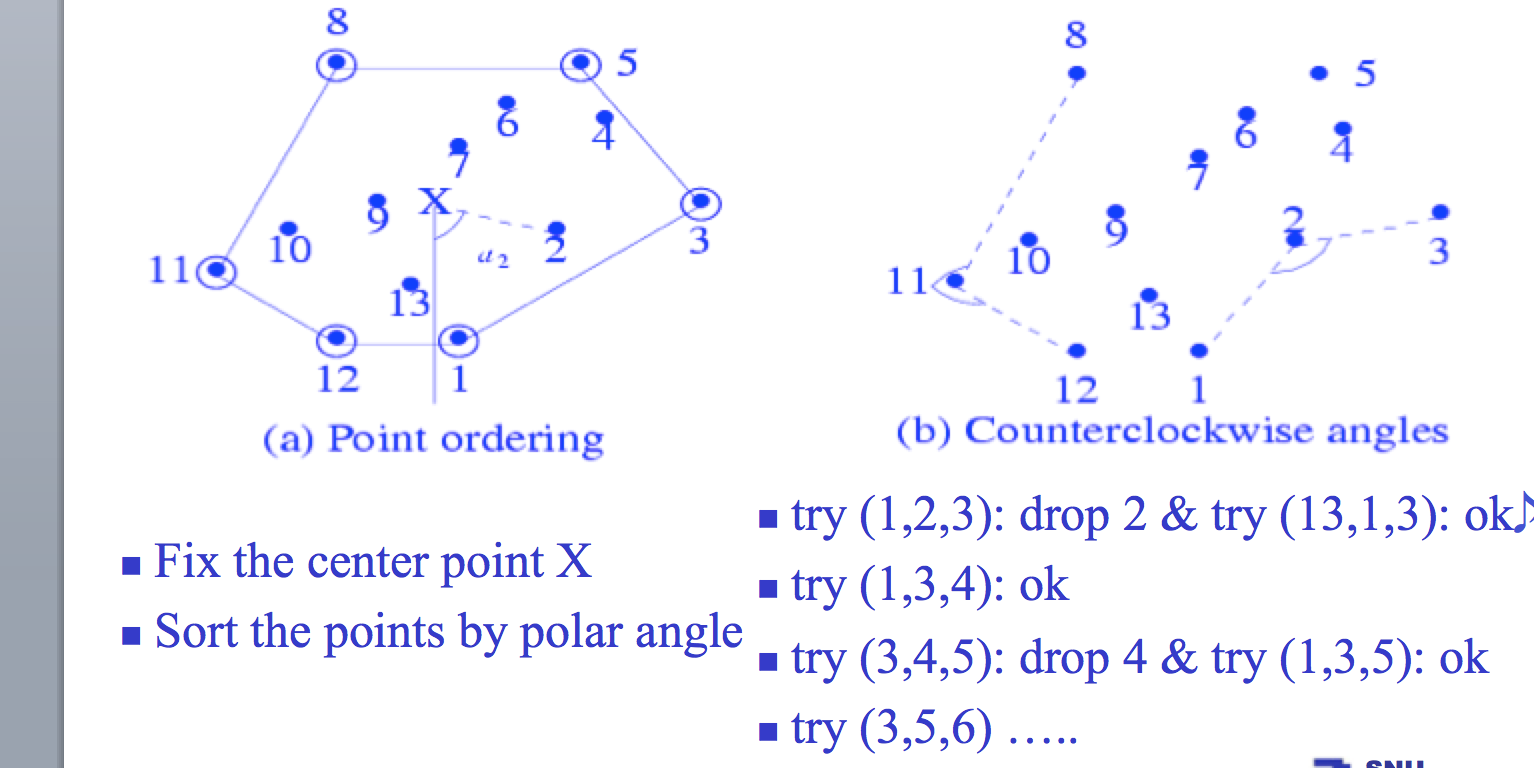
\includegraphics[scale=0.4]{pics/convex.png} \newline
\item Let p be the point that the smallest y-coordinate 
   (break a tie, if any, by selecting the one with largest x-coordinate)
   
\item use Law of cosines to calculate  angle formed by x, rx and rrx
\[
c^{2} = a^{2}+b^{2}-2ab\cos\lambda
\]

\begin{lstlisting}[frame=single, language=c++]
 for (x = p; rx = point to the right of x; x != rx) {
       rrx = point to the right of rx;
       if (angle formed by x, rx, and rrx is <=180 degrees) {
           delete rx from the list;
           rx = x; 
           x = point on left of rx;
       } 
       else { 
       x = rx; rx = rrx;}
   } 
\end{lstlisting}

\item For convex hull problem, you can use double link list to store all the extreme points. Because it need to use three consequence points to measure the degree to judge if it's less than 180 degrees. So double link list is the best data structure to use. 

\end{enumerate}


\subsection{Permutation and combination}
\begin{itemize}
\item repeated / unrepeated (Permutation/Combination)

\item repeated permutation: Three number, how many permutation $10^3$. Another Three position, For each position, you can select 10 options and fill it.  If three position, For each position, you can selet 2 options and fill it. You get powerset problem $2^3$ \{a,b, c\} all the subset. 

\item unrepeated permutation: $n! = factorial function$
\item unrepeated combination:  
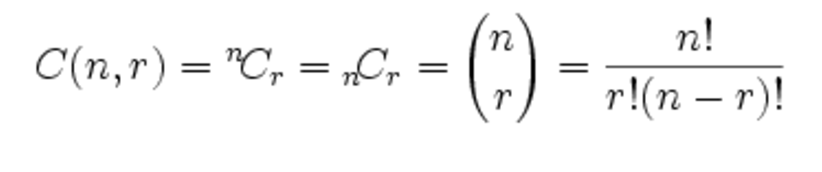
\includegraphics[scale=0.6]{pics/UC.png} \newline
\item repeated combination: 
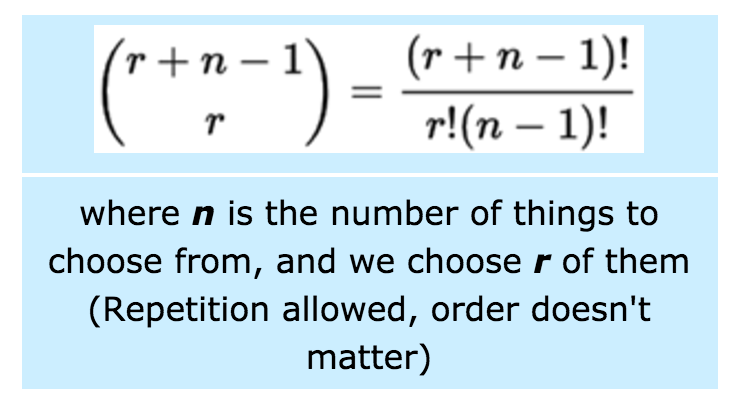
\includegraphics[scale=0.6]{pics/RC.png} \newline
\item detail can been seen here: https://www.mathsisfun.com/combinatorics/combinations-permutations.html

\end{itemize}

\subsection{solution space }
\begin{itemize}
\item why this basic conception is so important, Because you can use these four to describe solution space. repeated permutation can be use in 0/1 backpack problem.  LCS problem.  

\item nearest point pair's solution space is n*(n-1). It's $n^2$. A good hint is that it can be reduce $n*log(n)$. So We should consider D\&C (divide and conquer)

\item 0/1 packback's solution's space is $2^n$, A good hint is that I can be reduce to $n^c$. (c is constant) by dynamic programming. 

\item If there is not D\&C or DP, you have to use branch and bound or backtracking.  such as TSP travelling sales problem

\item If you need optimal answer, You need to traversal the whole solution space. ( such as TSP and 0/1 backpacking). If you don't need optimal answer, you don't need to do that, In these two conditions, you all need to \textbf{backtracking.}

\item Why I can't use DP to TSP, but I can use DP to 0/1?  

\end{itemize}

\begin{itemize}

\item recursion is a mathematical induction. 
\item modeling is mapping your problem to a abstract structure.
\begin{enumerate}
\item Permutation: arrangement, tour,ordering sequence
\item subset: cluster, collection, committee, group, packaging, selection
\item tree:hieracrchy, dominance, ancestor/descendant, taxonomy
\item graphs: network, circuit, web, relationship
\item points
\item polygon
\item string 
\end{enumerate}

\end{itemize}

\subsection{Usage of model \%}

\begin{itemize}
\item circular queue
\item hash
\item to know the last three digit. 
\end{itemize}

\section{Recursive}
\begin{itemize}

\item First, the inline specification on a function is just a hint. The compiler can (and often does) completely ignore the presence or absence of an inline qualifier. With that said, a compiler can inline a recursive function, much as it can unroll an infinite loop. It simply has to place a limit on the level to which it will "unroll" the function.



\item One recursive(Factorial),  Two recursive call( Hanoti) (Tree), Multi Recursive(Permutation)

\item result is single (FActorial), Result is many steps,(Hanoti) (Maze), Result is a set( permutation). you can see that 1) any recursive function should at least one input parameter, and this parameter should to be pass sub-problem. 2) for return value, it has two different kind, if result is single value, you should return a value, such as Factorial. If result is set(permutation) or many steps(in-order traversal of treeor Hanoi tree), you can declare your function as void. 3) Some functions need input another parameter, such as level information in the tree or position information in the permutation. 4) Base case can be understood differently, most of time base case is 0 or null, but for permutation, base case is i==n.  most subproblem, i decrease, but for permutation, for each subproblem i increase. 
\begin{enumerate}
\item single result 
\begin{lstlisting}[frame=single, language=c++]
int Factorial(int n){
if (n == 1) 
     return 1;
 return n*Factorial(n-1);
}
\end{lstlisting}
\item result is serial steps (Hanoti) DFS(Maze)
\begin{lstlisting}[frame=single, language=c++]
FUNCTION MoveTower(disk, source, dest, spare):
IF disk == 0, THEN:
    move disk from source to dest
ELSE:
    MoveTower(disk - 1, source, spare, dest)   // Step 1 above
    move disk from source to dest              // Step 2 above
    MoveTower(disk - 1, spare, dest, source)   // Step 3 above
END IF
\end{lstlisting}
Result is a set( permutation)

\end{enumerate}

\item permutation, It is also worth noting that when you make a recursive call, you advance down an individual branch of the tree, and an additional branch is added with every iteration of a 'for' or 'while' loop. One confusing thing about this problem is the second swap after the recursive call to permute. This can be interpreted as 'unswap,' and is required because the char array is passed by reference, not by value, and every time you swap elements in the array the change is visible down stream.

\begin{lstlisting}[frame=single, language=c++]
void permute(char a[], int i, int n){
   int j;
   if (i == n)
     cout << a << endl;
   else   {
       for (j = i; j <= n; j++)       {
          swap(a[i], a[j]);          
          permute(a, i+1, n);
          swap(a[i], a[j]);
       }
   }
} 
\end{lstlisting}

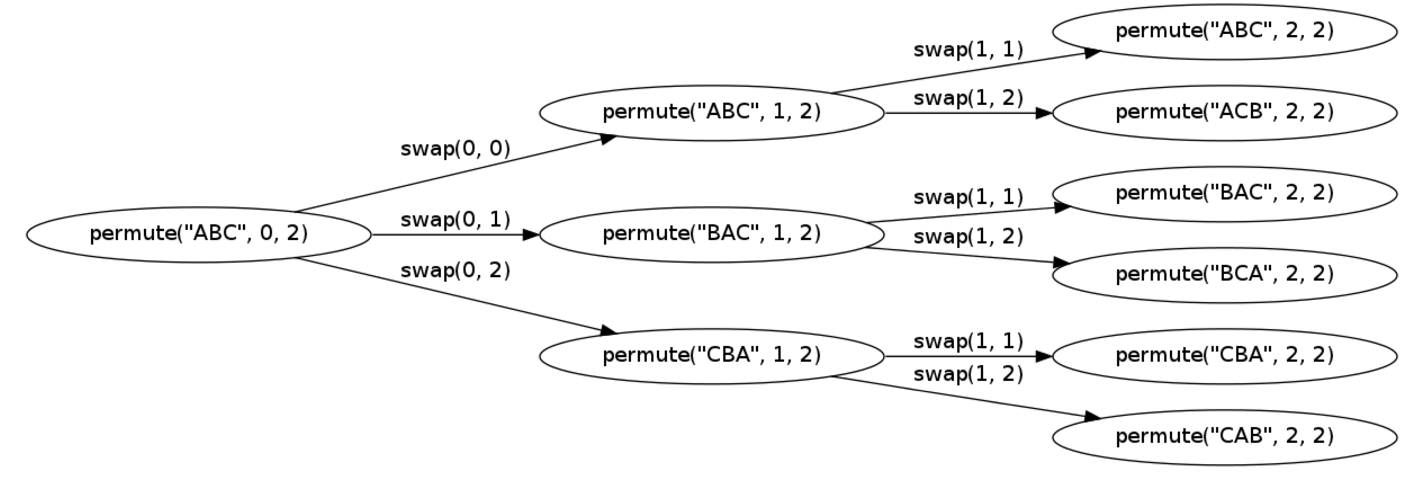
\includegraphics[scale=0.25]{pics/permutation.png}

\item It includes direct recursive and indirect recursive. direct recursive is R() call R() again in it's funciton body. It has two parts: \textbf{1)base and 2) recursive component}




\end{itemize}

\section{Sort}
\subsection{Simple sort}
\begin{itemize}
\item Write Max and Insert functions to help to organize your algorithm
\item All sort algorithm don't compare equal relationship. So some algorithm is Stable, and other is not stable
\item Bubble is simple source code stable sorting. 
\item All the sorting is from minimum to maximum.
\end{itemize}
 
\begin{enumerate}
\item for all sort comparsion, there is good ref website: https://www.toptal.com/developers/sorting-algorithms/selection-sort

\item Selection sort is an in-place comparison sort. O(n2). The algorithm finds the minimum value, swaps it with the value in the first position.  And repeat From the comparions presented here, one might conclude that selection sort should never be used. It does not adapt to the data in any way (notice that the four animations above run in lock step), so its runtime is always quadratic.

However, selection sort has the property of minimizing the number of swaps. In applications where the cost of swapping items is high, selection sort very well may be the algorithm of choice.
\begin{lstlisting}[frame=single, language=c++]
For(int size=n ;size>1;size--){
Int j = Max(a,size);
Swap(a[j],a[size-1]);
}
\end{lstlisting}

\item Insertion sort is suitable for small list and mostly sorted list. Although it is one of the elementary sorting algorithms with O(n2) worst-case time, insertion sort is the algorithm of choice either when the data is nearly sorted (because it is adaptive) or when the problem size is small (because it has low overhead).

For these reasons, and because it is also stable, insertion sort is often used as the recursive base case (when the problem size is small) for higher overhead divide-and-conquer sorting algorithms, such as merge sort or quick sort.

\begin{lstlisting}[frame=single, language=c++]
For(int I = 0;i<n;i++){
Int iv = a[i];
Insert(a,I, iv);
}
Insert(a[],int n,int lv){
For(int I = n-1;i>=0&&lv<a[i];i--)
    A[i+1]=a[i]  //move each element from tail to head one by one
A[i]  = lv;  //insert here. 
}
\end{lstlisting}

\item Bubble sort is stable 
\begin{lstlisting}[frame=single, language=c++]
For (int I = n;i>0;i--){
	For(int j= 0;j<I;j++)
		If(a[j]<a[j+1]) swap(a[j],a[j+1]);
}
\end{lstlisting}

\item Bubble sort can stops after reaching a sorted array. In the best case (already sorted), every insert requires constant time. So Bubble and insert can reach O(n) time in Best context. Bubble sort has many of the same properties as insertion sort, but has slightly higher overhead. In the case of nearly sorted data, bubble sort takes O(n) time, but requires at least 2 passes through the data (whereas insertion sort requires something more like 1 pass).

\item Selection sort only need O(n) write, so if write is expensive operation, you need to use it. 
\end{enumerate}  

\subsection{quick  sort}
\begin{itemize}
\item Three quick heapSort, MergeSort, quickSort. (Olog(n))
\item MergeSort need O(N) extra space. When you merge two lists, this shortcoming can be avoid

\item partition 
\begin{lstlisting}[frame=single, language=c++]
/* This function takes last element as pivot, places
   the pivot element at its correct position in sorted
    array, and places all smaller (smaller than pivot)
   to left of pivot and all greater elements to right
   of pivot */
partition (arr[], low, high){
    // pivot (Element to be placed at right position)
    pivot = arr[high];   
    i = (low - 1)  // Index of smaller element
    for (j = low; j <= high- 1; j++)    {
        // If current element is smaller than or
        // equal to pivot
        if (arr[j] <= pivot)        {
            i++;    // increment index of smaller element
            swap arr[i] and arr[j]
        }
    }
    swap arr[i + 1] and arr[high])
    return (i + 1)
}
\end{lstlisting}

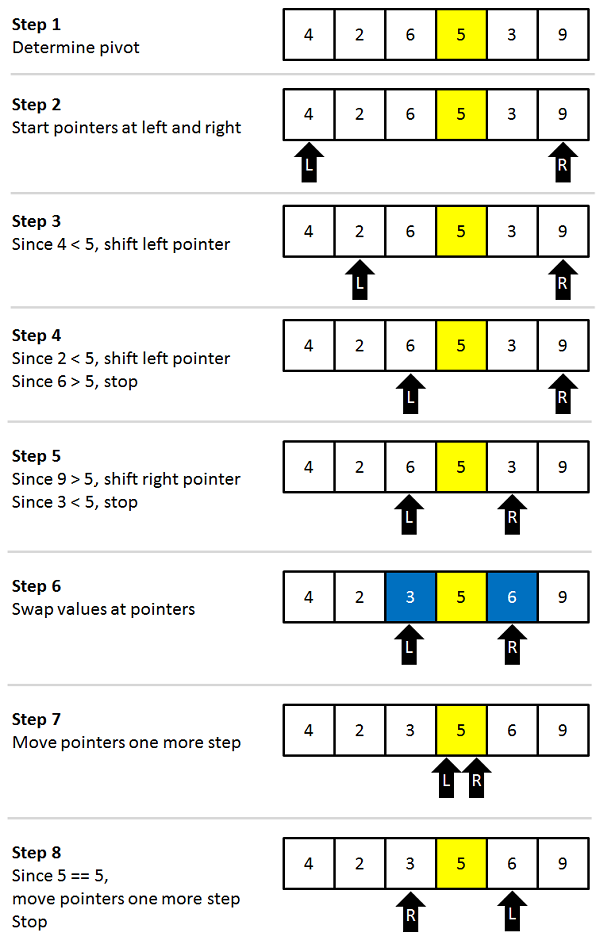
\includegraphics[scale=0.45]{pics/qsort1.png} \newline
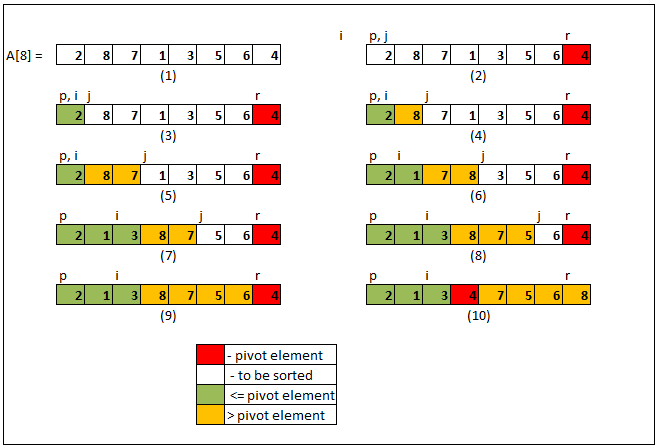
\includegraphics[scale=0.45]{pics/qsort2.png} \newline
\item Quick sort need random access ability.  

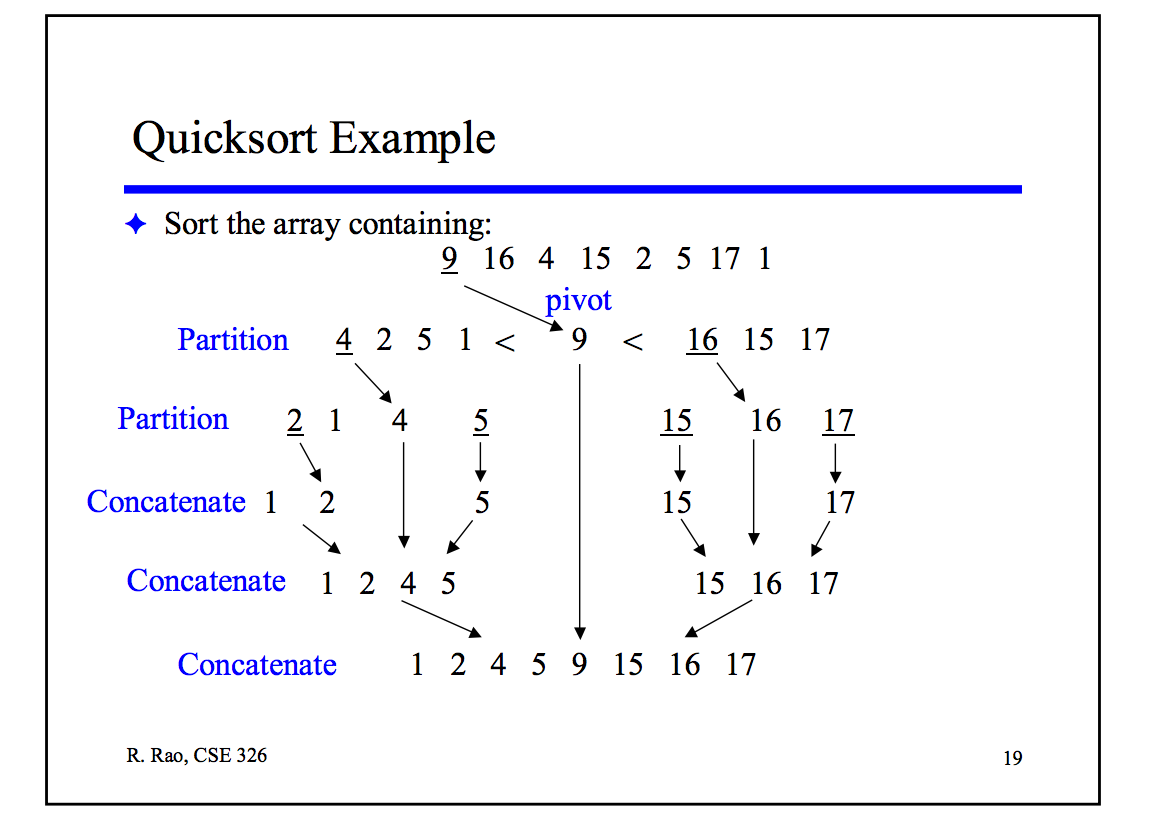
\includegraphics[scale=0.45]{pics/quick_sort.png} \newline


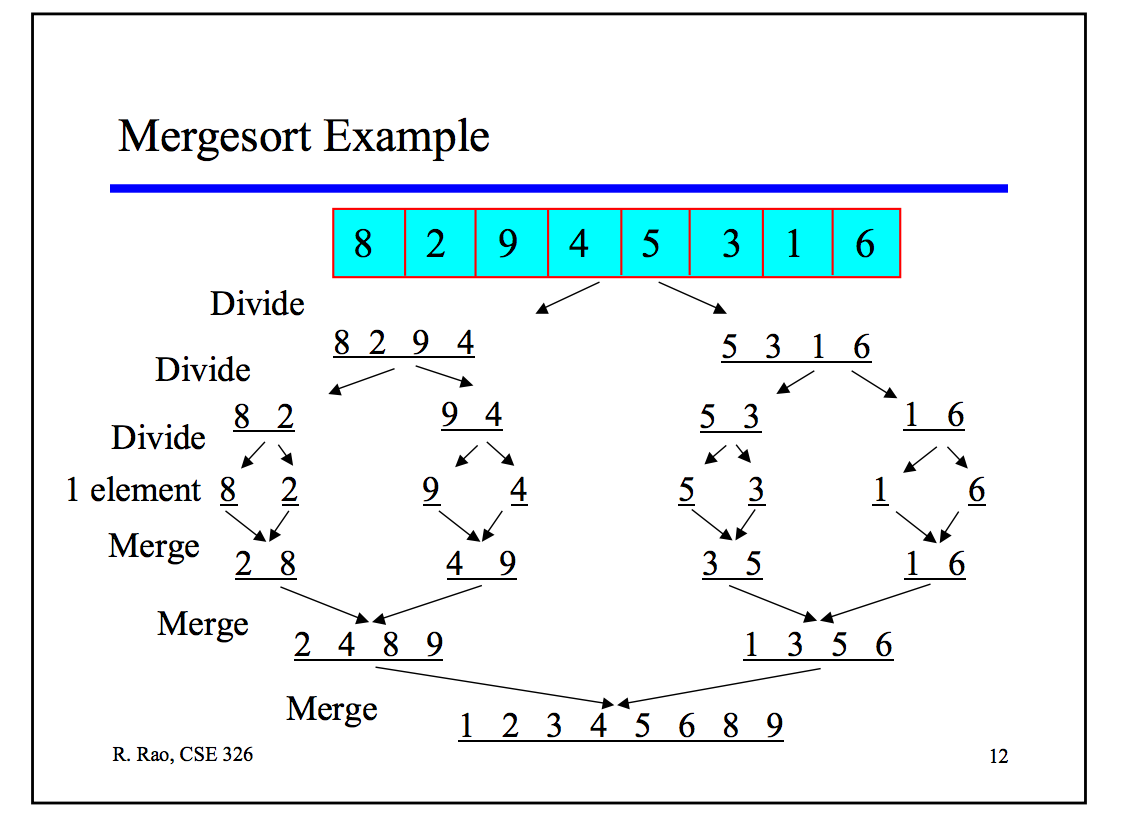
\includegraphics[scale=0.45]{pics/merge_sort.png} \newline



\end{itemize}

\subsection{Bucket and radix sort}
\begin{itemize}


\item Bucket sort is not comparison algorithm.  
\item we must know the maximum value in the unsorted array
\item How many objects in the unsorted array
\item If maximum value is not big, and objects is a lot. such as all student score (<100) in a school(1000). At this time, we can use Bucket sort. 
	
\item Firstly, we must know how to handle duplicates. Secondly,  Thirdly, we must have enough memory. If you sort telephone which will not allow duplicated value, you can build an bit array. And set bit 1 if there are number exist. It will save a lot of memories.   For duplicate, you can store a link in each bucket. (array item)

\item Radix sort is cousin of Bucksort BucketSort is more efficient for 'Dense' arrays, while RadixSort can handle sparse (well, not exactly sparse, but spaced-out) arrays well. Use \% operator to get radix each digit. 

\item $ 1\sim n^c-1$. $ 1\sim10^3-1 $  You can use 10 as radix, and sort it 3 times. 

\end{itemize}


\section{Greedy}
\begin{itemize} 

\item idea of Greedy
\begin{enumerate}
\item Solve a problem by making a sequence of decisions

\item Decisions are made one by one in some order

\item Each decision is made using a greedy criterion
At each stage we make a decision that appears to be the best at the time

\item A decision, once made, is (usually) not changed later
\end{enumerate}


\item	You need a \textbf{greedy criterion} to make a local decision 
\item 	Examples: makin change, 0/1 knappack,  activity selection (largest subset) sorted according to their finishing time, topological orders.  Dijkstra, Kruskal, prim and sollin

\item Applications: Container Loading, 0/1 knapsack problem, Topological sorting, Bipartite cover, Single-source shortest paths, Minimum-cost spanning trees. 

\end{itemize}

\subsection{application}
\begin{itemize}
\item  Machine Scheduling, \textbf{sort all task according to start time, and minheap of machine end time. }

\item Container Loading and 0/1 knapsack problem are different. For 0/1 knapsack problem, we consider the value and weight together,  For greed algorithm, it change time complexity from $2^{n}$to $n.log(n)$, but 583/600 is withing 10\%, so it's very practical algorithm.  Don't underestimate it. 

\item Topological sorting: 
\begin{verbatim}
1) Select any one among  vertices having no incoming edge
2) Put the node into the solution &  Remove the node and its outgoing edges from the graph
4) Repeat the above steps until no nodes remain

You need to InDegree[n] array to save and update all the vetex InDegree, and stack to store all the vetex which indegree is 0.  
\end{verbatim}


\item Bipartite-cover problems are NP-hard
\begin{verbatim}
A greedy method to develop a fast heuristic
Construct the cover A’ in stages
Select a vertex of A  using the greedy criterion:
Select a vertex of A that covers the largest # of uncovered vertices of B
\end{verbatim}

\item Dijkstra algorithm.  \newline
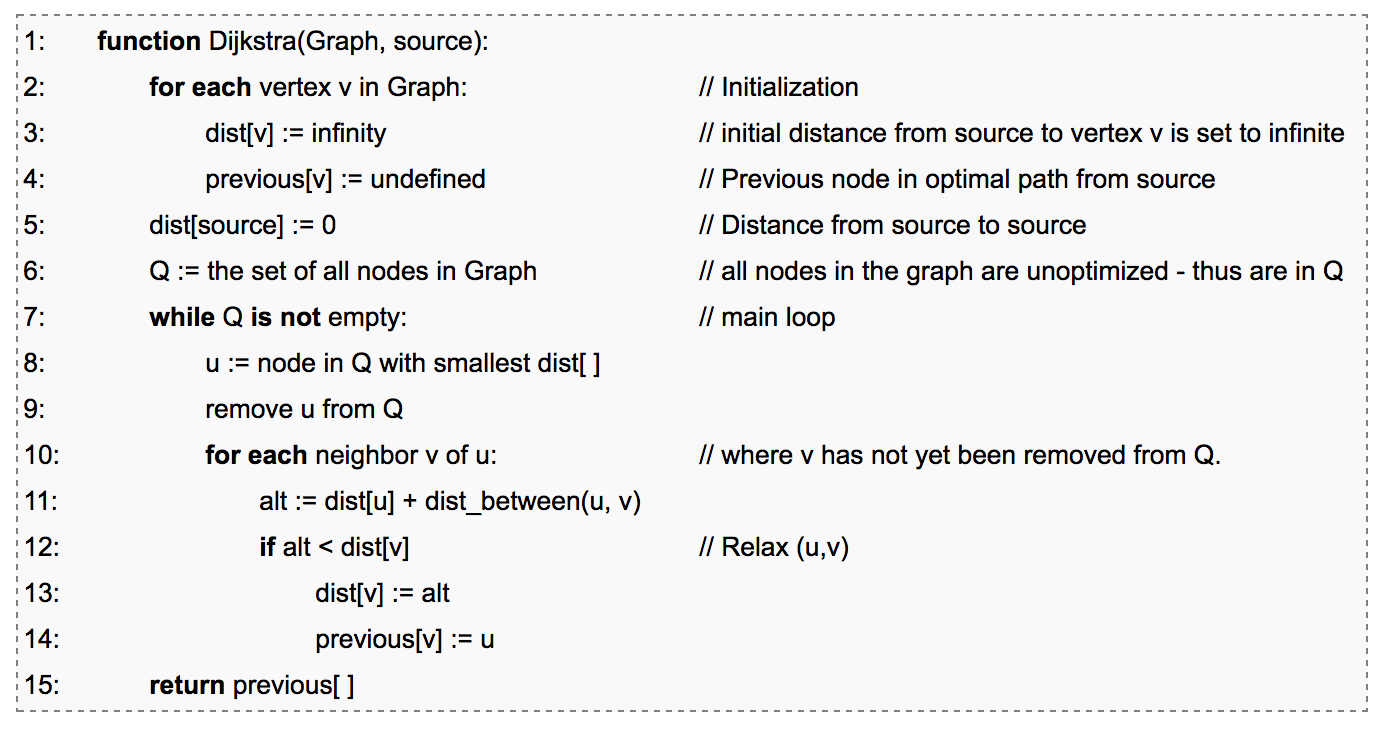
\includegraphics[scale=0.45]{pics/Dijkstra.png} \newline
\begin{enumerate}
\item The greedy idea lies in line 8
\item In line 8, it must shortest path to this vetex,  Because if it's not, There is shorter path, then, according to we select min in line 8, shorter one will be selected first, and this value HAS BEEN updated before. 
\item $O(n^{2})$
\item the shortest value is saved, it's also idea of dynamic programming.
\item Just like vertabi, you can think that they are the same. 
\end{enumerate}

\end{itemize}

\section{Divide Conquer}
\begin{itemize}
\item binary search:
\begin{enumerate}
\item only compare once, just  
\item avoid s+e overflow.
\item s will catch up e in the end, then break while loop 
\item check a[m] == k outside of while
\end{enumerate}

\begin{lstlisting}[frame=single, language=c++]
while(s<e) {
    //m=(s+e)/2;
    m = s/2+e/2 + s&e&1;
    if(a[m]<k)
        s = m+1;
    else 
       e = m;
}
if(a[m] == k) 
       return ture; 
\end{lstlisting}
\end{itemize} 

\section{Dynamic programming}
\begin{itemize}
\item The difference between dynamic programming and greedy algorithms is that with dynamic programming, the subproblems overlap. That means that by "memoizing" solutions to some subproblems, you can solve other subproblems more quickly.   


\item The top-down approach is generally recursive (but less efficient) and more intuitive to implement as it is often a matter of recognizing the pattern in an algorithm and refactoring it as a dynamic programming solution.

The bottom-up approach is generally iterative (and more efficient), but less intuitive and requires us to solve (and know!) the smaller problems first then use the combined values of the smaller problems for the larger solution.

We refer to top-down solutions as memoization and bottom-up as tabulation.

We’ll look at the reason for these terms below.

\item If we don’t need to solve all the problems and are just looking for the optimal solution, memoization is better.

If we do need to solve all the problems, that means we are going to make a lot of recursive calls, and tabulation is better.

The caveat is that memoization is generally more intuitive to implement especially when we don’t know the solution to subproblems, whereas tabulation requires us to know the solutions, or bottom, in advance, in order to build our way up.

\item In Divide and Conquer, the sub-problems are independent of each other while in case of Dynamic Programming, the sub-problems are not independent of each other (Solution of one sub-problem may be required to solve another sub-problem).

\item Divide and Conquer \\

Divide and Conquer works by dividing the problem into sub-problems, conquer each sub-problem recursively and combine these solutions. solves a problem by combining the solutions to  sub-problems

\begin{enumerate}
\item Partition the problem into non-overlapping sub-problems
\item Solve the sub-problems recursively
\item Combine their solutions to solve the original problem

\end{enumerate}



\item Dynamic Programming \\

Dynamic Programming is a technique for solving problems with overlapping subproblems. Each sub-problem is solved only once and the result of each sub-problem is stored in a table ( generally implemented as an array or a hash table) for future references. These sub-solutions may be used to obtain the original solution and the technique of storing the sub-problem solutions is known as memoization.

\item You may think of DP = recursion + re-use

A classic example to understand the difference would be to see both these approaches towards obtaining the nth fibonacci number. Check this material from MIT.

\item The principle of optimality \\
No matter what the first decision, the remaining decisions must be optimal with respect to the state that results from this first decision
Dynamic programming may be used only when the principle of optimality holds. Useful when the sub-problems are overlapping

Solve an optimization problem by caching  sub-problem solutions rather than recomputing them

\begin{enumerate}
\item Verify that the principle of optimality holds  \newline
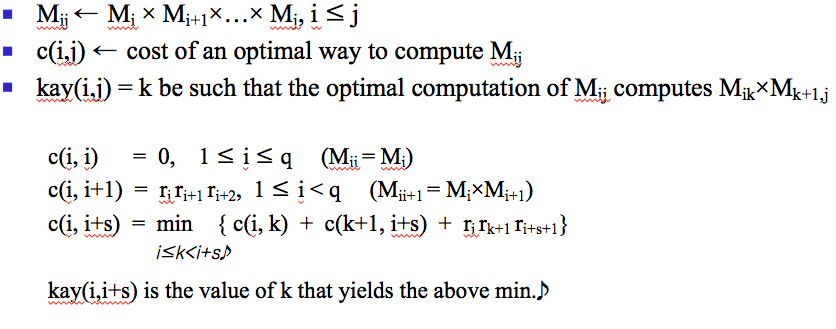
\includegraphics[scale=0.45]{pics/Recurrence.png} \newline

\item Set up the dynamic-programming recurrence equations
\item Solve the dynamic-programming recurrence equations for the value of the optimal solution
\item Perform a traceback step in which the solution itself is constructed
\end{enumerate}


Recursive
Simple, intuitive code
Unless care is taken to avoid recomputing previously computed values, the recursive program will have prohibitive complexity

Iterative
Not require additional space for the recursion stack
To minimize run time overheads, and hence to reduce actual run time, dynamic programming recurrences are almost always solved iteratively    (no recursion).


Longest Increasing Subsequence

i is index, i+1 change it to length. because interface need lengh, but inside we use. index, you have to pay attention here.

\begin{lstlisting}[numbers=none]

int input[6] = {50, 3, 10, 7, 40, 80};

int lis(int* p, int num, int* m){
	
	if (m[num-1] != -1)
	return m[num-1];
	
	cout<<"doing "<<num<<endl;
	if (num ==1){
		return 1;
	}
	int result = 0;
	int value = p[num-1];
	
	for(int i = num-2; i>=0;i--){
		int temp = 0;
		int child = lis(p, i+1,m); 
		// i is index, 
		//i+1 change it to length. 
		//because interface need lengh, but inside we use 
		//index, you have to pay attention here.
		
		if (value>p[i]){
			temp = child +1;
		}
		else{
			temp = child;
		}
		
		if (temp>result){
			result = temp;
		}
	}
	m[num-1] = result;
	return result;
}

int main() {
	
	int m[6] = {1,-1, -1, -1, -1, -1};
	int result = lis(input, 6, m);
	cout<<result<<endl;
	
	return 0;
}
\end{lstlisting}



\begin{lstlisting}[numbers=none]
vector<string> input = {"ab", "abc", "cd", "def", "abcd", "ef" , "c"};
string target = "abcdef";

vector<vector<string> > ac(string target, const vector<string> & in ){
	if (target.size() == 0){
		return vector<vector<string>> {{}};
	}
	
	vector<vector<string>> last_result;
	
	for(auto i: input){
		if (target.find(i) == 0){
			string sub = target;
			sub.erase(0, i.size());
			vector<vector<string>> re = ac(sub, in);
			for(auto j : re){
				j.push_back(i);
				last_result.push_back(j);
			}
		}
	}
	return last_result;
}

int main() 
{ 
	string test("aabb");
	cout<<test.find("aa");
	test.erase(0,2);
	cout<<test.size()<<endl;
	vector<vector<string>> result = ac(target, input);
	
	for(auto i: result ){
		for(auto j: i){
			cout<< j<<" ";
		}
		cout<<endl;
	}
	
	cout<< "hello"<<endl;
	return 0; 
}

\end{lstlisting} 

\subsubsection{Top-down}

\item \textbf{There are three kinds of questions: Can, ALL, Min}, below is min questions.  

\begin{lstlisting}[numbers=none]
int arr[] = {1, 3, 5, 8, 9, 2, 6, 7, 6, 8, 9};

int minj(int arr[], int last){
	
	cout<<"calculate..."<<last<<endl;
	
	if (last ==1 && arr[last]>=1){
		return 1;
	}
	
	
	int min = last;
	for(int i = last-1; i>=0;i--){
		if (i+arr[i]>=last){
			int step = 1+minj(arr,i);
			if( step<min){
				min = step;
			}
		}    
	}
	return min;
}
\end{lstlisting} 

\item below is getting all questions.  
\begin{lstlisting}[numbers=none]
int arr[] = {1, 3, 5, 8, 9, 2, 6, 7, 6, 8, 9};

vector<vector<int> >  minj(int arr[], int last){	
	if (last ==1 && arr[last]>=1){
		vector<int> v1 = {1};
		vector<vector<int> > v = {v1};
		return v;
	}	
	vector<vector<int> > result;
	
	int min = last;
	for(int i = last-1; i>=0;i--){
		if (i+arr[i]>=last){
			vector<vector<int> > result1 = minj(arr,i);
			for(auto e: result1){
				e.push_back(arr[i]);
				result.push_back(e);
			}
		}
	}
	return result;
}

\end{lstlisting} 

\item below is getting Can questions.  
\begin{lstlisting}[numbers=none]
int arr[] = {1, 3, 5, 8, 9, 2, 6, 7, 6, 8, 9};

bool  minj(int arr[], int last){
	
	
	if (last ==1 && arr[last]>=1){
		return true;
	}
	
	bool result = false;
	
	for(int i = last-1; i>=0;i--){
		if (i+arr[i]>=last){
			result = true && minj(arr,i);
			if(result)
			break;
		}
	}
	return result;
}
\end{lstlisting} 

\subsubsection{bottom-up}
\item resolve can problem.

\end{itemize}

\section{backtracing and branch and bound}
\begin{itemize}
\item Backtracking:
\begin{enumerate}
\item It is used to find all possible solutions available to the problem.
\item It traverse tree by DFS(Depth First Search).
\item It realizes that it has made a bad choice \& undoes the last choice by backing up.
\item It search the state space tree until it found a solution.
\item It involves feasibility function.
\end{enumerate}


\item Branch-and-Bound
\begin{enumerate}
\item It is used to solve optimization problem.
\item It may traverse the tree in any manner, DFS or BFS.
\item It realizes that it already has a better optimal solution that the pre-solution leads to so it abandons that pre-solution.
\item It completely searches the state space tree to get optimal solution.
\item It involves bounding function.

\item Searches a solution space that is often organized as a tree (like backtracking)
\item Usually searches a tree in a breadth-first / least-cost manner (unlike backtracking)

\end{enumerate}

\item Difference between DFS and backtracking is:
\begin{enumerate}
\item Backtracking is a more general purpose algorithm. Depth-First search is a specific form of backtracking related to searching tree or graphic structures.  
\item For a problem, answer space can be described as a tree graphic structure, such as 0/1 backpack problem. at this time, backtracking use DFS to search the answer space, and use questions related condition to prune the sub-tree and com back. So in this way, you can think backtracking = DFS+prune. 

\item For mouse raze, because, prune is "no next neighbor", just like DFS, so DFS and backtracking are the totally same.
\end{enumerate}

\item Difference between branch-bound  and backtracking is about size
\begin{enumerate}
\item backtracking use stack and only add one child each time, so it use less memory compared with branch-bound
\item branch-bound store all possible child in queue, so if answer is near root, it will find answer quickly. 

\item win in size, but lose in time. backtracking will 1) find answer slowly, 2) branch-bound will find optimal answer. 
\end{enumerate}

\item A example can be see in ref PPT.  container and ship problems. 

\end{itemize}


\chapter{Code snippet}
\section{STL}
\subsection{New int}
\begin{itemize}
	\item two methods to trim string.
	
\begin{lstlisting}[numbers=none]
const std::string WHITESPACE = " \n\r\t\f\v";
string ltrim(const string& str){
	size_t pos = str.find_first_not_of(WHITESPACE);
	if (pos == string::npos){
		return "";
	}
	else{
		return str.substr(pos);
	}
}
		
string rtrim(string& str){
	auto pos = find_if(str.rbegin(),str.rend(), [](char c){ 
		return !isspace(c, locale::classic());}
		);
		
	str.erase(pos.base(), str.end());
	return str;
}
\end{lstlisting}
	\begin{description}
		\item[Line 2] ltrim uses \texttt{find\_first\_not\_of}, then return a position. The first parameter of substr is beginning position and second parameter of substr is length. 
		\item[Line 12] rtrim uses generic stl algorithm \texttt{find\_if}. It return a iterator. \textbf{Using auto type when it will be assigned by iterator.}. Learn how to write lambda function.  Erase function does modification in place. 
	\end{description}
	
	\item token
\begin{lstlisting}[numbers=none]
	str1="zhao,yao,c++";
	stringstream s1(str1);
	unordered_set<string> sv2;
		
	string str_part;
	while(getline(s1, str_part, ',')){
		sv2.insert(str_part)
	}
\end{lstlisting}
	
	\begin{description}
		\item[Source code] stringstream+getline can make token much easier.
	\end{description}

\item That is usage of unique\_ptr in vector. 

\begin{lstlisting}[numbers=none]
template <typename T>
void vector<T>::push_back(const T& value){
	cout<<"call push_back"<<endl;
	
	if(index_>=capacity_){
		capacity_ *=2;
		cout<<"new capacity"<<endl;
		unique_ptr<int[]> temp = make_unique<T[]>(capacity_);
		T* ps = data.get();
		copy(ps, ps+capacity_, temp.get());
		data = move(temp);
	}
	
	data[index_] = value;
	index_++;
}
\end{lstlisting}

	
	\item Useful function of str.
\begin{lstlisting}[numbers=none]
	str=to_string(123);
	str.erase(0,1) //delete the first letter
	str.pop_back() //delete the last letter
\end{lstlisting}
	
	
	\item Find all occurrences in a collection
\begin{lstlisting}[numbers=none]
void All(const string& str){
	auto ll = [](char c){
		return isdigit(c);
		};
			
	auto p = find_if(str.begin(), str.end(), ll);
	while(p != str.end()){
		cout<<distance(str.begin(),p)<<endl;
		p = find_if(p+1, str.end(), ll);
	}
}
\end{lstlisting}
	\begin{description}
		\item[line 2] define lambda and give it a name. Because we will reuse it.
		\item[line 6] \textbf{For string, there are two ways to index a position: index(size\_t) and iterator(auto)}. If you use find\_if, then later you have to use \texttt{str.end()}, you can't use \texttt{string::npos}.
		\item[line 8] distance is calculated by the second parameter - the first parameter.
		\item[Source code] First get initialize p, the while(p != end), last p+1. That is very useful source code pattern. 
	\end{description}


\item use of generate
\begin{lstlisting}[numbers=none]
srand(time(NULL));
vector<int> v1;

generate_n(back_inserter(v1, begin(v1)) , 5,
[](){return rand()%10;} 
	);
	
	for(auto i: v1){
		cout<<i<<endl;
	}
\end{lstlisting}
\begin{description}
	\item[line 1] \#include ctime and cstdlib. srand(time(NULL)) is normal routine before you use rand.
	\item[line 4] You can use begin(v1) function, it's better version. please use back\_inserter(v1, begin(v1)) here. it will change assignment into push\_back. The similar two options are inserter and front\_inserter. 

\end{description}



\item two matrix multiply
\begin{lstlisting}[numbers=none]
int inner_product(int row, int col, int num, const vector<vector<int>> &v1, 
const vector<vector<int>> &v2){
	int sum = 0;
	for (int i =0 ;i<num ;i++){
		sum += v1[row][i]*v2[i][col];
	}
	return sum;
}

int main(){
	vector<vector<int> > m1 = {{1,2,3}, {4, 5, 6}};
	vector<vector<int> >m2 = { {1,2}, {3,4}, {5,6}};
	int m1_row = m1.size();
	int m1_col = m1[0].size();
	int m2_row = m2.size();
	int m2_col = m2[0].size();
	vector<vector<int> > result = {{0,0}, {0,0}};
	
	for(int i = 0;i<m1_row;i++){
		for(int j= 0;j<m2_col;j++){
			int element = inner_product(i, j,3, m1, m2); 
			result[i][j] = element;
		}
	}
	
	for(auto i: result){
		for(auto j: i){
			cout<<j<<endl;
		}
	}
	return 0;
}
\end{lstlisting}

\begin{description}
	\item[line ] matrix support list initialization.
	
	\item[line ] \textbf{In this questions, inner\_product is key point to resolve. First, get atomic operation and change it into a function. Then, design this function parameter and in the end, design outside enviroment to call this automic function. This is very an important strategy} 
	
	\item[line ] two for(auto.. ) can be use to print out matrix very easily.
\end{description}

\item sprial print a matrix
\begin{lstlisting}[numbers=none]
int
print_out (int rb, int re, int cb, int ce, bool isrow, bool positive,
const vector < vector < int >>&v)
{
	if (isrow){
		if (positive){
			for (int i = cb; i <= ce; i++){
				cout << v[rb][i]<<',';
			}
		}
		else{
			for (int i = ce; i >= cb; i--){
				cout << v[re][i]<<',';
			}
		}
	}
	else
	{
		if (positive){
			for (int i = rb; i <= re; i++){
				cout << v[i][ce]<<',';
			}
		}
		else{
			for (int i = re; i >= rb; i--){
				cout << v[i][cb]<<',';
			}
		}
	}
}

int main ()
{
	vector < vector < int >>m1 = { {1, 2, 3}, {4, 5, 6}, {7, 8, 9} };
	int row = m1.size()-1;
	int col = m1[0].size()-1;
	
	int rb = 0, re = row, cb = 0, ce = col;
	int isrow = 1;
	int positive = 1;
	while (rb <= re && cb <= ce){
		
		if (isrow == 1 && positive == 1)
		{
			print_out (rb, re, cb, ce, isrow, positive,m1);
			rb++;
			isrow = 0;
			positive =1;
		}
		if (isrow == 0 && positive == 1)
		{
			print_out (rb, re, cb, ce, isrow, positive,m1);
			ce--;
			isrow = 1;
			positive = 0;
		}
		if (isrow == 1 && positive == 0)
		{
			print_out (rb, re, cb, ce, isrow, positive,m1);
			re--;
			isrow = 0;
			positive = 0;
		}
		if (isrow == 0 && positive == 0)
		{
			print_out (rb, re, cb, ce, isrow, positive,m1);
			cb++;
			isrow = 1;
			positive = 1;
		}
	}
	return 0;
}	
	
\end{lstlisting}		
	
\begin{description}
	\item[line ] \textbf{In this questions, print\_out is key. }
	\item[line ] \textbf{Get atomic operation, print\_out, design the interface of this key function. after it, design the context which use this key function: print\_out. In this context, usually involve a loop and change boundary parameter.}
	
	\item[line ] rb, re, cb, ce very good clue, once you found these four parameters, then this question becomes easier. another two useful flag is isrow and positive. 
\end{description}


\end{itemize}



\ifx \allfiles \undefined
%\end{CJK*}
\end{document}
\fi
